% PrismSpace: System Flow, Architecture, DB Schema & Algorithm Presentation
\documentclass[aspectratio=169,10pt]{beamer}
\usetheme{Madrid}
\usecolortheme{default}
\usefonttheme{professionalfonts}
\usepackage[T1]{fontenc}
\usepackage{lmodern}
\usepackage{amsmath,amssymb}
\usepackage{booktabs}
\usepackage{tikz}
\usepackage{adjustbox}
\usepackage{tcolorbox}
\tcbuselibrary{skins}
\usepackage{fontawesome5}
\usepackage{tabularx}
\usepackage{array}
\usepackage{colortbl}
\usetikzlibrary{arrows.meta,positioning,fit,backgrounds,calc,shadows,shapes.geometric,tikzmark}

\providecommand{\pk}[1]{\textbf{#1}}
\providecommand{\idx}[1]{\textit{#1}}
\providecommand{\comp}[1]{\texttt{#1}}

% Lavender Color Palette for Professional Headers & Visual Flow
\definecolor{lavenderDark}{RGB}{76, 51, 122}      % #4C337A - Deep Royal Lavender for Frametitles, Banners, Headers
\definecolor{lavenderDeep}{RGB}{58, 36, 96}       % #3A2460 - High-contrast lavender for text on light backgrounds
\definecolor{lavenderMedium}{RGB}{124, 98, 173}   % #7C62AD - Medium Lavender for Subheaders, Footers, Accents
\definecolor{lavenderLight}{RGB}{243, 239, 252}   % #F3EFFC - Soft Lavender Mist for fills and backgrounds
\definecolor{lavenderBorder}{RGB}{186, 168, 224}  % #BAA8E0 - Soft Lavender border
\definecolor{lavenderAccent}{RGB}{150, 120, 205}  % #9678CD - Accent lilac for highlights & bullets

% PrismSpace Supporting Palette
\definecolor{bannerGreen}{RGB}{76, 51, 122}
\definecolor{prismNavy}{RGB}{76, 51, 122}
\definecolor{prismBlue}{RGB}{124, 98, 173}
\definecolor{prismTeal}{RGB}{22,138,114}
\definecolor{prismMint}{RGB}{235,248,245}
\definecolor{prismGold}{RGB}{217,154,34}
\definecolor{prismDark}{RGB}{23,32,42}
\definecolor{prismLight}{RGB}{248,247,252}
\definecolor{prismIndigo}{RGB}{76, 51, 122}
\definecolor{prismSlate}{RGB}{102,112,133}
\definecolor{cardBg}{RGB}{255,255,255}

% Harmonious pastel node fills
\definecolor{cInput}{RGB}{231,233,236}
\definecolor{cStem}{RGB}{220,214,247}
\definecolor{cStage1}{RGB}{191,232,213}
\definecolor{cStage2}{RGB}{246,213,138}
\definecolor{cStage3}{RGB}{242,184,181}
\definecolor{cStage4}{RGB}{191,227,242}
\definecolor{cHead}{RGB}{216,197,232}
\definecolor{cOutput}{RGB}{234,207,213}

% Execution-core fills
\definecolor{cTask}{RGB}{231,233,236}
\definecolor{cPlanner}{RGB}{207,199,242}
\definecolor{cDispatch}{RGB}{169,220,235}
\definecolor{cReact}{RGB}{169,222,200}
\definecolor{cTool}{RGB}{244,213,141}
\definecolor{cSafety}{RGB}{240,170,167}
\definecolor{cMemory}{RGB}{214,185,230}
\definecolor{cDeliverable}{RGB}{185,222,210}

% Beamer Palette Settings - Lavender Theme
\setbeamercolor{structure}{fg=lavenderDark}
\setbeamercolor{background canvas}{bg=prismLight}
\setbeamercolor{normal text}{fg=prismDark,bg=prismLight}
\setbeamercolor{frametitle}{bg=lavenderDark,fg=white}
\setbeamercolor{title}{fg=lavenderDark}
\setbeamercolor{author}{fg=lavenderMedium}
\setbeamercolor{institute}{fg=gray}
\setbeamercolor{date}{fg=gray}

\setbeamercolor{block title}{bg=lavenderDark,fg=white}
\setbeamercolor{block body}{bg=cardBg,fg=prismDark}
\setbeamercolor{block title alerted}{bg=prismGold!90!black,fg=white}
\setbeamercolor{block body alerted}{bg=prismGold!10,fg=prismDark}
\setbeamercolor{block title example}{bg=lavenderMedium,fg=white}
\setbeamercolor{block body example}{bg=lavenderLight,fg=prismDark}

\setbeamertemplate{navigation symbols}{}

% Professional Header and Footer
\setbeamercolor{author in head/foot}{bg=lavenderDark, fg=white}
\setbeamercolor{title in head/foot}{bg=lavenderMedium, fg=white}
\setbeamercolor{date in head/foot}{bg=lavenderDark, fg=white}
\setbeamertemplate{footline}
{
  \leavevmode%
  \hbox{%
  \begin{beamercolorbox}[wd=.28\paperwidth,ht=2.5ex,dp=1.1ex,center]{author in head/foot}%
    \usebeamerfont{author in head/foot}\textbf{Group 01} $\cdot$ CSE, CEK
  \end{beamercolorbox}%
  \begin{beamercolorbox}[wd=.48\paperwidth,ht=2.5ex,dp=1.1ex,center]{title in head/foot}%
    \usebeamerfont{title in head/foot}\textbf{PrismSpace}: Architecture, Flow, DB \& Swarm Algorithm
  \end{beamercolorbox}%
  \begin{beamercolorbox}[wd=.24\paperwidth,ht=2.5ex,dp=1.1ex,right]{date in head/foot}%
    \usebeamerfont{date in head/foot}\insertframenumber{} / \inserttotalframenumber\hspace*{2ex} 
  \end{beamercolorbox}}%
  \vskip0pt%
}

\setbeamertemplate{itemize item}{\color{lavenderAccent}$\blacktriangleright$}
\setbeamertemplate{itemize subitem}{\color{lavenderMedium}$\bullet$}
\setbeamertemplate{itemize subsubitem}{\color{prismGold}$-$}

% Title Metadata
\title[PrismSpace]{\textbf{\LARGE PrismSpace}}
\subtitle{\large System Flow, Multi-Layer Architecture, Browser DB Schema \& Swarm Algorithms}
\author[Group 01]{
  \textbf{Nobin Sijo} \and \textbf{Pranav P} \and \textbf{Prasanth P} \and \textbf{Sankar Narayan S}
}
\institute[CEK]{
  \textbf{Department of Computer Science \& Engineering}\\
  College of Engineering, Karunagappally
}
\date{\today}

\begin{document}

% =============================================================================
% SLIDE 1: TITLE SLIDE
% =============================================================================
\begin{frame}[plain]
\begin{tikzpicture}[remember picture,overlay]
  % 1. Top Lavender Banner
  \node[
    rounded corners=5pt,
    fill=lavenderDark,
    drop shadow={shadow xshift=1.5pt, shadow yshift=-2.0pt, opacity=0.35},
    minimum width=15.2cm,
    minimum height=0.98cm,
    inner sep=0pt
  ] at ([yshift=-0.78cm]current page.north) {};

  \node[text=white, font=\bfseries\fontsize{13.5}{16}\selectfont] at ([yshift=-0.78cm]current page.north) {
    PRISMSPACE - INTELLIGENT MULTI-AGENT PLATFORM
  };

  % 2. College Emblem
  \node at ([yshift=-1.95cm]current page.north) {
    
\includegraphics[height=0.95cm]{cek-logo.png}
  };

  % 3. Department & College Text
  \node[font=\footnotesize, align=center] at ([yshift=-2.82cm]current page.north) {
    \textbf{Dept. of Computer Science \& Engineering}\\[0.12em]
    College of Engineering, Karunagappally
  };

  % 4. Project Group Header
  \node[font=\large\bfseries, text=lavenderDark] at ([yshift=-3.55cm]current page.north) {
    Project Group 01
  };

  % 5. Students & Register Numbers Table
  \node[font=\small] at ([yshift=-4.60cm]current page.north) {
    \begin{tabular}{l@{\hspace{3.4cm}}l}
      \textbf{NOBIN SIJO}        & KNP23CS082 \\
      \textbf{PRANAV P}          & KNP23CS085 \\
      \textbf{PRASANTH P}        & KNP23CS086 \\
      \textbf{SANKAR NARAYAN S}  & KNP23CS094
    \end{tabular}
  };

  % 6. Horizontal Lavender Accent Line
  \draw[lavenderDark, line width=0.9pt] ([xshift=1.6cm, yshift=-5.58cm]current page.north west) -- ([xshift=-1.6cm, yshift=-5.58cm]current page.north east);

  % 7. Project Coordinator & Guide Details
  \node[align=center, font=\footnotesize] at ([yshift=-6.70cm]current page.north) {
    {\color{lavenderDark}\textit{Project Coordinator \& Guide}}\\[0.25em]
    \textbf{\small Dr. Leena Silvoster}\\[0.12em]
    Associate Professor\\[0.08em]
    College of Engineering, Karunagappally
  };
\end{tikzpicture}
\end{frame}

% =============================================================================
% SLIDE 2: INTRODUCTION
% =============================================================================
\section{Introduction}

\begin{frame}[c]{01. Introduction: PrismSpace Web Platform}
\centering
\begin{minipage}{0.94\linewidth}
\begin{tcolorbox}[
  enhanced, arc=5pt, colframe=lavenderDark!80, colback=lavenderLight!25,
  boxrule=0.9pt,
  left=14pt, right=14pt, top=12pt, bottom=12pt
]
\fontsize{8.6}{12.6}\selectfont\sffamily\color{lavenderDeep}
  \textbf{\fontsize{10.2}{13.0}\selectfont\color{lavenderDark}PrismSpace} is an interactive, \textbf{web-based multi-agent intelligence platform} and workspace website that allows users to orchestrate autonomous AI swarms directly from modern web browsers. It converts natural-language user goals into dependency-aware \textbf{Directed Acyclic Graphs (DAGs)} for parallel sub-task execution. Built as a responsive web application (Next.js 15, React 19) accessible from any browser with zero local setup, it features an interactive visual DAG swarm visualizer with real-time token and step streaming. The platform pairs Groq, OpenAI, and NVIDIA NIM with standardized tool connectivity via Model Context Protocol (MCP), while storing all session state locally in client-side IndexedDB (\texttt{PrismDB}) with human-in-the-loop approval gates for privacy and safety.
\end{tcolorbox}
\end{minipage}
\end{frame}

% =============================================================================
% SLIDE 3: PROBLEM STATEMENT
% =============================================================================
\section{Problem Statement}

\begin{frame}[t]{02. Problem Statement: Core Challenges in AI Agent Systems}
\vspace{0.25em}

\centering
\begin{minipage}{0.95\linewidth}
\fontsize{7.8}{10.0}\selectfont

\begin{enumerate}\setlength{\itemsep}{7.5pt}\setlength{\leftmargin}{0.28in}
  \item \textbf{Monolithic LLM Bottleneck \& High Cost:} Traditional platforms route all planning, reasoning, and tool use through a single massive LLM, causing severe prompt bloat, high latency, and $3\times$ higher inference expenses.\\
  \textcolor{prismTeal!90!black}{\textbf{\faArrowCircleRight\ PrismSpace Solution:}} Dynamically routes sub-tasks to cost- and latency-optimal models (Groq for rapid inference, OpenAI/NIM for complex reasoning).

  \item \textbf{Sequential \& Rigid Task Execution:} Existing agent chains run strictly in linear sequence; independent sub-tasks wait needlessly in line, and a single step crash causes total pipeline collapse.\\
  \textcolor{prismTeal!90!black}{\textbf{\faArrowCircleRight\ PrismSpace Solution:}} Deconstructs goals into dynamic Directed Acyclic Graphs (DAGs) to execute independent tasks in parallel ($K \le 3$) with isolated fault recovery.

  \item \textbf{Fragmented Tool Silos \& Black-Box Runs:} Proprietary integrations isolate essential productivity tools (Gmail, Drive, Terminal, Local Files), while users remain blind during long runs with no status logs.\\
  \textcolor{prismTeal!90!black}{\textbf{\faArrowCircleRight\ PrismSpace Solution:}} Standardizes all tool connections via Model Context Protocol (MCP) paired with real-time execution telemetry and progress logs.

  \item \textbf{Safety Hazards \& Cloud Data Lock-in:} Autonomous agents execute irreversible actions (sending emails, modifying files) without oversight, while cloud databases expose private user data.\\
  \textcolor{prismTeal!90!black}{\textbf{\faArrowCircleRight\ PrismSpace Solution:}} Enforces Human-in-the-Loop (HITL) approval gates, ORPO alignment, and zero-latency local browser database storage (\texttt{PrismDB}).
\end{enumerate}

\end{minipage}
\end{frame}

% =============================================================================
% SLIDE 3: COMPARATIVE ANALYSIS (EXISTING PLATFORMS VS. PRISMSPACE)
% =============================================================================
\section{Comparative Analysis}

\begin{frame}[t]{03. Comparative Analysis: Existing Platforms vs. PrismSpace}
\vspace{-0.44em}

% Top subtitle banner
\centering
\begin{tcolorbox}[
  enhanced, colback=lavenderDark!90, colframe=lavenderDark, arc=3pt,
  boxrule=0.5pt, width=0.98\linewidth, top=1.4pt, bottom=1.4pt, left=8pt, right=8pt,
  halign=center
]
  \textcolor{white}{\fontsize{6.6}{8.0}\selectfont\sffamily
  \textbf{Architectural Benchmark:} Evaluating PrismSpace against industry-standard conversational AI, autonomous agents, and swarm frameworks.}
\end{tcolorbox}

\vspace{-0.46em}

% Comparison Matrix Table
\begin{tcolorbox}[
  enhanced, arc=3.5pt, colframe=lavenderDark!75, colback=white,
  boxrule=0.60pt, left=3pt, right=3pt, top=1.0pt, bottom=1.0pt, width=0.98\linewidth
]
\setlength{\tabcolsep}{3.0pt}
\fontsize{5.0}{6.0}\selectfont
\renewcommand{\arraystretch}{1.10}
\begin{tabularx}{\linewidth}{>{\raggedright\arraybackslash\bfseries\color{lavenderDark}}m{2.35cm} | >{\centering\arraybackslash}m{2.35cm} | >{\centering\arraybackslash}m{2.35cm} | >{\centering\arraybackslash}m{2.35cm} | >{\raggedright\arraybackslash\columncolor{prismMint!75}}X}
\hline
\rowcolor{lavenderLight!80}
\centering\textbf{\fontsize{5.4}{6.6}\selectfont Capability Dimension} &
\begin{minipage}{2.25cm}\centering\vspace{1pt}
  
\includegraphics[height=0.34cm]{logos/chatgpt.png}\\[1pt]
  \textbf{\fontsize{5.5}{6.6}\selectfont ChatGPT Web}\\\fontsize{4.4}{5.2}\selectfont (OpenAI)
\vspace{1pt}\end{minipage} &
\begin{minipage}{2.25cm}\centering\vspace{1pt}
  
\includegraphics[height=0.34cm]{logos/autogpt.png}\\[1pt]
  \textbf{\fontsize{5.5}{6.6}\selectfont AutoGPT}\\\fontsize{4.4}{5.2}\selectfont (Autonomous Loop)
\vspace{1pt}\end{minipage} &
\begin{minipage}{2.25cm}\centering\vspace{1pt}
  
\includegraphics[height=0.34cm]{logos/crewai.png}\\[1pt]
  \textbf{\fontsize{5.5}{6.6}\selectfont CrewAI}\\\fontsize{4.4}{5.2}\selectfont (Multi-Agent Swarm)
\vspace{1pt}\end{minipage} &
\begin{minipage}{\linewidth}\centering\vspace{1pt}
  {\fontsize{6.5}{7.5}\selectfont\color{prismTeal}\faProjectDiagram}\enspace
  \textbf{\fontsize{6.0}{7.2}\selectfont\color{lavenderDark}PrismSpace (Ours)}\\[1pt]
  \fontsize{4.6}{5.4}\selectfont\bfseries\color{prismTeal!90!black}Local Multi-Agent Platform
\vspace{1pt}\end{minipage} \\
\hline

\textbf{Execution Topology} &
Linear single-thread prompt dialog &
Unbounded recursive loop (risk of infinite loops) &
Sequential or static hierarchical agent chains &
\textbf{\color{prismTeal!90!black}Dynamic DAG Scheduling:} Parallel execution ($K \le 3$, join barriers) \\
\hline

\textbf{Model Strategy \& Routing} &
Vendor locked (single OpenAI model per session) &
Single model API backend (typically GPT-4) &
Statically configured per agent persona &
\textbf{\color{prismTeal!90!black}Dynamic Multi-Model Router:} Routes Groq, OpenAI, NIM by latency/cost \\
\hline

\textbf{Tool Connectivity Protocol} &
Proprietary OpenAI Plugins \& Function Calls &
Custom Python scripts \& local shell commands &
LangChain tool wrappers (rigid contracts) &
\textbf{\color{prismTeal!90!black}Model Context Protocol (MCP):} Standardized servers (Gmail, Drive, FS, Web) \\
\hline

\textbf{Observability \& Streaming} &
Text token stream only (internal steps opaque) &
Terminal CLI logs only; zero visual graph &
Terminal text traces; server-side execution &
\textbf{\color{prismTeal!90!black}Live SSE Stream + Visual DAG:} Real-time node state and telemetry \\
\hline

\textbf{Safety \& Quality Control} &
Closed cloud content filter; no user approval gate &
Fixed step budgets; no output verification &
Agent self-critique (incurs token overhead) &
\textbf{\color{prismTeal!90!black}HITL Approval Gates + ORPO:} High-risk tasks paused; preference aligned \\
\hline

\textbf{Persistence \& Privacy} &
Remote cloud storage (privacy \& latency exposure) &
Local filesystem artifacts; no structured database &
Cloud DB or ephemeral in-memory state &
\textbf{\color{prismTeal!90!black}Local-First PrismDB:} Zero-latency browser IndexedDB (\texttt{useLiveQuery()}) \\
\hline
\end{tabularx}
\end{tcolorbox}

\vspace{-0.40em}
\begin{tcolorbox}[
  enhanced, arc=2.5pt, colframe=prismTeal!75!black, colback=prismMint!50,
  boxrule=0.5pt, left=4pt, right=4pt, top=1.0pt, bottom=1.0pt, width=0.98\linewidth
]
\fontsize{4.8}{5.8}\selectfont\color{prismDark}
While ChatGPT is optimized for single-model dialog and frameworks like CrewAI/AutoGPT for Python-scripted execution, \textbf{PrismSpace} uniquely unifies \textbf{dynamic DAG planning}, \textbf{open MCP tools}, \textbf{multi-model routing}, and \textbf{local-first privacy} in a reactive workspace.
\end{tcolorbox}

\end{frame}

% =============================================================================
% SLIDE 4: OBJECTIVES
% =============================================================================
\section{Objectives}

\begin{frame}[t]{04. Project Objectives}
\vspace{0.55em}
  \begin{minipage}{0.94\linewidth}
  \fontsize{8.6}{11.2}\selectfont
  \begin{enumerate}\setlength{\itemsep}{12pt}\setlength{\leftmargin}{0.34in}
    \item \textbf{Context-Aware Task Planning:} Convert everyday user goals (communication, file management, daily schedules) and technical requests into structured Directed Acyclic Graphs (DAGs) for organized, dependency-safe execution.
    \item \textbf{Intelligent Model \& Agent Routing:} Dynamically route each sub-task to the most suitable Large Language Model (LLM) backend and dispatch specialized, context-aware agents in parallel.
    \item \textbf{Practical Tool Execution via MCP:} Connect agents to everyday productivity tools and development utilities (Gmail, Google Drive, Filesystem, Terminal CLI, GitHub) through the Model Context Protocol (MCP), accompanied by live Server-Sent Events (SSE) updates.
    \item \textbf{Safety Verification \& Local Persistence:} Validate outputs with human approval checkpoints and Odds Ratio Preference Optimization (ORPO), storing results reactively in local IndexedDB (Indexed Database: \texttt{PrismDB}).
  \end{enumerate}
  \end{minipage}
\end{frame}

% =============================================================================
% SLIDE 5: AT A GLANCE (FIGURE 1.0) - UNDERSTAND IN 3 SLIDES CENTERPIECE
% =============================================================================
\section{System Overview}

\begin{frame}[t]{05. PrismSpace Workflow (Figure 1.0)}
\vspace{-0.15em}
\centering
\adjustbox{max width=0.98\linewidth, max height=0.74\textheight}{%
\begin{tikzpicture}[
    x=1cm, y=1cm,
    font=\sffamily,
    stepbox/.style={
        rectangle, draw=lavenderDark!80, line width=0.85pt, fill=white,
        rounded corners=4pt, inner sep=4pt, align=center,
        drop shadow={shadow xshift=1pt, shadow yshift=-1pt, opacity=0.2}
    },
    flowarr/.style={
        -{Stealth[scale=0.85]}, line width=1.1pt, draw=lavenderDark!90
    },
    dashloop/.style={
        -{Stealth[scale=0.75]}, line width=0.85pt, dashed, draw=prismGold!90!black
    }
]

    % Step 1: User Request
    \node [stepbox, fill=cInput, text width=2.5cm] (b1) at (-6.2, 0) {
        \textbf{\fontsize{8.2}{9.8}\selectfont\color{lavenderDark}1. User Request}\\[0.22em]
        \fontsize{6.2}{7.4}\selectfont
        $\bullet$ Daily or tech goal\\
        $\bullet$ Email, docs, or code\\
        $\bullet$ Context and history
    };

    % Step 2: Supervisor & Router
    \node [stepbox, fill=cPlanner, text width=2.6cm] (b2) at (-2.8, 0) {
        \textbf{\fontsize{8.2}{9.8}\selectfont\color{lavenderDark}2. Task Router}\\[0.22em]
        \fontsize{6.2}{7.4}\selectfont
        $\bullet$ Request type\\
        $\bullet$ Best model selection\\
        $\bullet$ Task planning
    };

    % Step 3: Swarm Agents and responsibilities
    \node [stepbox, fill=cReact, text width=3.05cm] (b3) at (0.8, 1.25) {
        \textbf{\fontsize{8.2}{9.8}\selectfont\color{lavenderDark}3. Swarm Agents}\\[0.18em]
        \fontsize{5.7}{6.8}\selectfont
        {\color{prismIndigo}\faProjectDiagram}\; \textbf{Planner:} makes task plan\\
        {\color{prismBlue}\faSearch}\; \textbf{Assistant:} \mbox{handles daily tasks}\\
        {\color{prismTeal}\faCode}\; \textbf{Coder:} edits code\\
        {\color{purple!75!black}\faClipboardCheck}\; \textbf{Validator:} checks results
    };

    % Step 4: MCP servers with project connections
    \node [stepbox, fill=cTool, text width=3.05cm] (b4) at (0.8, -1.25) {
        \textbf{\fontsize{8.2}{9.8}\selectfont\color{lavenderDark}4. MCP Servers}\\[0.15em]
        \fontsize{5.7}{6.8}\selectfont
        {\color{red!70!black}\faGoogle}\; \textbf{Gmail:} email management\\
        {\color{prismBlue}\faGoogleDrive}\; \textbf{Google Drive:} documents\\
        {\color{prismGold!90!black}\faFolderOpen}\; \textbf{Filesystem:} local files\\
        {\color{prismTeal}\faTerminal}\; \textbf{Tools:} terminal, web
    };

    % Step 5: Validator & Safety Gate
    \node [stepbox, fill=cSafety, text width=2.6cm] (b5) at (4.4, 0) {
        \textbf{\fontsize{8.2}{9.8}\selectfont\color{lavenderDark}5. Validation}\\[0.22em]
        \fontsize{6.2}{7.4}\selectfont
        $\bullet$ Policy check\\
        $\bullet$ Human approval\\
        $\bullet$ ORPO score
    };

    % Step 6: Real Outputs
    \node [stepbox, fill=cDeliverable, text width=3.35cm] (b6) at (8.15, 0) {
        \textbf{\fontsize{8.2}{9.8}\selectfont\color{lavenderDark}6. Real Outputs}\\[0.18em]
        \fontsize{5.7}{6.8}\selectfont
        {\color{red!70!black}\faEnvelope}\; \textbf{Gmail:} sent emails \& drafts\\
        {\color{prismBlue}\faGoogleDrive}\; \textbf{Drive:} docs \& spreadsheets\\
        {\color{prismTeal}\faCode}\; \textbf{Files:} code edits \& artifacts\\
        {\color{prismGold!90!black}\faTerminal}\; \textbf{Tools:} CLI runs \& web data
    };

    % Connect main flow
    \draw [flowarr] (b1) -- (b2);
    \draw [flowarr] (b2.east) -- ++(0.3, 0) |- (b3.west);
    \draw [flowarr] (b2.east) -- ++(0.3, 0) |- (b4.west);
    \draw [{Stealth[scale=0.8]}-{Stealth[scale=0.8]}, line width=1.0pt, draw=prismTeal] (b3) -- (b4);
    \draw [flowarr] (b3.east) -| ++(0.3, -1.25) -- (b5.west);
    \draw [flowarr] (b4.east) -| ++(0.3, 1.25) -- (b5.west);
    \draw [flowarr] (b5) -- (b6);

    % Feedback Loop - lifted clear of the Swarm Agents box
    \draw [dashloop] (b5.north) -- ++(0, 1.75) -| node[pos=0.5, above=2pt, font=\fontsize{6.2}{7.5}\selectfont\bfseries\color{prismGold!90!black}]{Validation Feedback \& Retry Loop} (b2.north);

\end{tikzpicture}%
}
\vspace{0.2em}
\begin{tcolorbox}[
  enhanced, arc=3pt, colframe=lavenderDark!65, colback=lavenderLight!35,
  boxrule=0.6pt, left=4pt, right=4pt, top=1.5pt, bottom=1.5pt
]
\centering\fontsize{4.8}{5.8}\selectfont\color{lavenderDark}
\textbf{Figure 1.0: PrismSpace Workflow} $\;\vert\;$ 
\textbf{DAG} = Directed Acyclic Graph $\;\vert\;$ 
\textbf{MCP} = Model Context Protocol $\;\vert\;$ 
\textbf{ORPO} = Odds Ratio Preference Optimization $\;\vert\;$ 
\textbf{SSE} = Server-Sent Events
\end{tcolorbox}
\end{frame}

% =============================================================================
% SLIDE 6: SYSTEM DESIGN
% =============================================================================
\section{System Design}

\begin{frame}[t]{06. System Design Principles}
\vspace{-0.15em}
\begin{itemize}\footnotesize\setlength{\itemsep}{4pt}
  \item \textbf{Layered Decoupling:} Separates the React client UI, FastAPI bridge, and foundation LLMs (each layer has one clear role).
  \item \textbf{Dynamic DAG Scheduling:} Runs dependent sub-tasks in parallel ($K \le 3$; additional tasks are queued) for daily and technical workflows.
  \item \textbf{Standardized Protocol (MCP):} Uses open JSON-RPC tool contracts (a common way for agents and tools to communicate).
  \item \textbf{Human-in-the-Loop:} Sensitive operations require explicit user approval (a safety checkpoint before execution).
  \item \textbf{Local IndexedDB (\texttt{PrismDB}):} ACID browser storage (reliable local data) for sessions, tasks, tool history, and files.
  \item \textbf{Reactive Subscriptions:} Dexie \texttt{useLiveQuery()} updates the UI automatically when data changes.
  \item \textbf{Server-Sent Events (SSE):} Streams tokens and agent telemetry over persistent HTTP (live one-way updates).
  \item \textbf{Calibrated Preference Gating:} ORPO ranks and filters outputs to improve quality and safety.
  \item \textbf{Design Philosophy:} Context-aware, sandboxed, and observable multi-agent workspace (safe and traceable by design).
\end{itemize}
\end{frame}

% =============================================================================
% SLIDE 7: AGENT LIFECYCLE, MCP INTEGRATION & RUNTIME FLOW
% =============================================================================
% Copyright 2026 Nobin Sijo (NobinSijo7T).
% SPDX-License-Identifier: Apache-2.0
% Agent Lifecycle & MCP Integration Slide Frame

\begin{frame}[t]{07. Agent Lifecycle, MCP Integration \& Runtime Flow in PrismSpace}
\vspace{-0.45em}

% Top Subtitle Banner (Compact, zero extra vertical margins)
\centering
\begin{tcolorbox}[
  enhanced,
  colback=lavenderDark!95,
  colframe=lavenderDark,
  arc=2.5pt,
  boxrule=0.5pt,
  width=0.99\linewidth,
  top=1.6pt, bottom=1.6pt, left=6pt, right=6pt,
  before=\vspace{0pt}, after=\vspace{1pt},
  halign=center
]
  \textcolor{white}{\fontsize{5.8}{7.0}\selectfont\sffamily
    \textbf{Runtime Orchestration \& Tool Architecture:} State-machine lifecycle with Human-in-the-Loop (HITL) safety gates, bi-directional MCP tool discovery, and real-time Server-Sent Events (SSE) telemetry.
  }
\end{tcolorbox}

\vspace{0.02cm}

\begin{columns}[t]

% ==================== LEFT COLUMN: AGENT LIFECYCLE ====================
\begin{column}{0.485\textwidth}
\centering
{\fontsize{7.2}{8.2}\selectfont\textbf{\color{lavenderDark}\faProjectDiagram\ Agent Lifecycle \& State Flow}}
\vspace{0.04cm}

\adjustbox{max width=\linewidth, max height=0.57\textheight, keepaspectratio}{%
\begin{tikzpicture}[
  x=1cm, y=1cm,
  font=\sffamily,
  statenode/.style={
    rectangle, rounded corners=3.5pt,
    line width=0.8pt, inner sep=3.0pt,
    align=center, font=\fontsize{6.2}{7.2}\selectfont\bfseries,
    drop shadow={opacity=0.10, shadow xshift=0.5pt, shadow yshift=-0.5pt}
  },
  decisionnode/.style={
    diamond, aspect=1.8,
    draw=statusApprove!90, fill=statusApprove!18, text=black,
    line width=0.85pt, inner sep=1.5pt,
    minimum width=2.5cm, align=center,
    font=\fontsize{5.6}{6.6}\selectfont\bfseries,
    drop shadow={opacity=0.10, shadow xshift=0.5pt, shadow yshift=-0.5pt}
  },
  terminode/.style={
    rectangle, rounded corners=3pt,
    line width=0.8pt, inner sep=2.5pt,
    minimum width=1.95cm, minimum height=0.48cm,
    align=center, font=\fontsize{5.4}{6.4}\selectfont\bfseries,
    drop shadow={opacity=0.08, shadow xshift=0.5pt, shadow yshift=-0.5pt}
  },
  arr/.style={-{Stealth[scale=0.75]}, line width=0.85pt, draw=black!75},
  greenarr/.style={-{Stealth[scale=0.75]}, line width=0.85pt, draw=statusComplete!90!black},
  redarr/.style={-{Stealth[scale=0.75]}, line width=0.85pt, draw=statusFail!90!black}
]

% Colors
\definecolor{statusInit}{RGB}{70, 130, 218}
\definecolor{statusPlan}{RGB}{22, 138, 114}
\definecolor{statusRun}{RGB}{230, 126, 34}
\definecolor{statusApprove}{RGB}{217, 154, 34}
\definecolor{statusComplete}{RGB}{39, 174, 96}
\definecolor{statusFail}{RGB}{217, 54, 54}
\definecolor{statusCancel}{RGB}{120, 140, 155}
\definecolor{prismTeal}{RGB}{22, 138, 114}
\definecolor{prismMint}{RGB}{235, 248, 245}

% Agent Lifecycle Nodes
\node[statenode, draw=statusInit!85, fill=statusInit!14, minimum width=4.9cm, minimum height=0.52cm] (init) at (0, 2.50) {
  \faRocket\ \textbf{INITIALIZING}\\[-0.08em]
  {\fontsize{4.9}{5.9}\selectfont\normalfont Run ID assigned $\cdot$ Session token $\cdot$ Background worker setup}
};

\node[statenode, draw=statusPlan!85, fill=statusPlan!14, minimum width=4.9cm, minimum height=0.52cm] (plan) at (0, 1.62) {
  \faSitemap\ \textbf{PLANNING}\\[-0.08em]
  {\fontsize{4.9}{5.9}\selectfont\normalfont Intent routing $\cdot$ Dependency DAG $\cdot$ Spawn workers $(K \le 3)$}
};

\node[decisionnode] (hitl) at (0, 0.76) {
  \faUserShield\ HITL Gate\\
  {\fontsize{4.5}{5.3}\selectfont Destructive op?}
};

\node[statenode, draw=statusApprove!85, fill=statusApprove!16, minimum width=2.90cm, minimum height=0.58cm] (approval) at (-1.75, -0.30) {
  \faHandPaper\ \textbf{AWAITING\_APPROVAL}\\[-0.08em]
  {\fontsize{4.7}{5.7}\selectfont\normalfont Operator prompt (300s timer)}
};

\node[statenode, draw=statusRun!85, fill=statusRun!16, minimum width=2.90cm, minimum height=0.58cm] (running) at (1.75, -0.30) {
  \faCogs\ \textbf{RUNNING}\\[-0.08em]
  {\fontsize{4.7}{5.7}\selectfont\normalfont ReAct loop via Provider API}
};

% Terminal States (Planar row - ZERO overlap)
\node[terminode, draw=statusCancel!85, fill=statusCancel!15] (cancelled) at (-2.15, -1.34) {
  \faBan\ \textbf{CANCELLED}\\[-0.08em]
  {\fontsize{4.5}{5.3}\selectfont\normalfont Operator rejected}
};

\node[terminode, draw=statusFail!85, fill=statusFail!15] (failed) at (0, -1.34) {
  \faTimesCircle\ \textbf{FAILED}\\[-0.08em]
  {\fontsize{4.5}{5.3}\selectfont\normalfont Error / Timeout}
};

\node[terminode, draw=statusComplete!85, fill=statusComplete!15] (completed) at (2.15, -1.34) {
  \faCheckDouble\ \textbf{COMPLETED}\\[-0.08em]
  {\fontsize{4.5}{5.3}\selectfont\normalfont Result stored \& streamed}
};

% Non-intersecting Arrow Flows
\draw[arr] (init) -- (plan);
\draw[arr] (plan) -- (hitl);

\draw[arr] (hitl.west) -| node[pos=0.35, above, font=\fontsize{4.9}{5.9}\selectfont\bfseries\color{statusApprove!90!black}]{YES} (approval.north);
\draw[arr] (hitl.east) -| node[pos=0.35, above, font=\fontsize{4.9}{5.9}\selectfont\bfseries\color{statusComplete!90!black}]{NO} (running.north);

% Approval to Running (Clear horizontal connector)
\draw[greenarr] (approval.east) -- node[above, font=\fontsize{4.6}{5.6}\selectfont\bfseries\color{statusComplete!90!black}]{Approved} (running.west);

% Downward paths from Approval
\draw[arr] ([xshift=-0.45cm]approval.south) -- node[left=1pt, font=\fontsize{4.5}{5.3}\selectfont\color{statusCancel!90!black}]{Reject} (cancelled.north);
\draw[redarr] ([xshift=0.35cm]approval.south) -- node[above right=-2pt, font=\fontsize{4.3}{5.1}\selectfont\color{statusFail!90!black}]{Timeout} ([xshift=-0.40cm]failed.north);

% Downward paths from Running
\draw[greenarr] ([xshift=0.45cm]running.south) -- node[right=1pt, font=\fontsize{4.5}{5.3}\selectfont\color{statusComplete!90!black}]{Success} (completed.north);
\draw[redarr] ([xshift=-0.35cm]running.south) -- node[above left=-2pt, font=\fontsize{4.3}{5.1}\selectfont\color{statusFail!90!black}]{Error} ([xshift=0.40cm]failed.north);

% Runtime Metrics & Telemetry Card (Single-line crisp bullets with explicit vertical spacing)
\node[rectangle, rounded corners=3pt, fill=prismMint, draw=prismTeal!70, line width=0.60pt,
      text width=6.05cm, align=left, inner sep=3.2pt] (metrics) at (0, -2.25) {%
  {\fontsize{4.8}{6.0}\selectfont
  \textbf{\color{prismTeal!90!black}\faChartLine\ Runtime Telemetry \& State Persistence:}\\[2pt]
  $\bullet$\enspace \textbf{SSE Stream:} Live token streaming \& status events over HTTP\\[1.5pt]
  $\bullet$\enspace \textbf{Telemetry (0.5s):} Step latency, token consumption \& model cost\\[1.5pt]
  $\bullet$\enspace \textbf{ACID Persistence:} JSONL execution traces saved to \texttt{PrismDB}\par}%
};

\end{tikzpicture}%
}
\end{column}

% ==================== RIGHT COLUMN: MCP INTEGRATION ====================
\begin{column}{0.485\textwidth}
\centering
{\fontsize{7.2}{8.2}\selectfont\textbf{\color{lavenderDark}\faPlug\ MCP Tool Integration \& Runtime Flow}}
\vspace{0.04cm}

\adjustbox{max width=\linewidth, max height=0.57\textheight, keepaspectratio}{%
\begin{tikzpicture}[
  x=1cm, y=1cm,
  font=\sffamily,
  mcpbox/.style={
    rectangle, rounded corners=3.5pt,
    line width=0.8pt, inner sep=3.0pt,
    align=center, font=\fontsize{6.2}{7.2}\selectfont\bfseries,
    drop shadow={opacity=0.10, shadow xshift=0.5pt, shadow yshift=-0.5pt}
  },
  toolbox/.style={
    rectangle, rounded corners=2.5pt,
    draw=prismGold!80, fill=prismGold!12, text=black,
    line width=0.65pt, inner sep=2.0pt,
    minimum width=1.95cm, minimum height=0.42cm,
    align=center, font=\fontsize{4.9}{5.9}\selectfont
  },
  arr/.style={-{Stealth[scale=0.75]}, line width=0.85pt, draw=black!75},
  dasharr/.style={-{Stealth[scale=0.65]}, line width=0.75pt, draw=mcpBlue!90, dashed}
]

% Colors
\definecolor{mcpBlue}{RGB}{41, 128, 185}
\definecolor{mcpGreen}{RGB}{39, 174, 96}
\definecolor{prismGold}{RGB}{217, 154, 34}
\definecolor{statusApprove}{RGB}{217, 154, 34}

% Stage 1: MCP Configuration & Loader
\node[mcpbox, draw=mcpBlue!85, fill=mcpBlue!12, minimum width=6.2cm, minimum height=0.52cm] (config) at (0, 2.50) {
  \faFileCode\ \textbf{MCP Configuration \& Transports}\\[-0.08em]
  {\fontsize{4.9}{5.9}\selectfont\normalfont \texttt{mcp\_servers.json} $\cdot$ Stdio / SSE JSON-RPC $\cdot$ Masked env tokens}
};

% Stage 2: Orchestration Context
\node[mcpbox, draw=mcpBlue!85, fill=mcpBlue!12, minimum width=6.2cm, minimum height=0.52cm] (context) at (0, 1.62) {
  \faBrain\ \textbf{Orchestration Context \& Dynamic Discovery}\\[-0.08em]
  {\fontsize{4.9}{5.9}\selectfont\normalfont Servers parsed $\rightarrow$ Tool schemas injected into LLM system prompt}
};

% Stage 3: MCP Tool Grid (2 rows x 3 columns)
\node[toolbox] (browser) at (-2.10, 0.86) {
  \faGlobe\ \textbf{Browser}\\[-0.05em]
  {\fontsize{4.4}{5.2}\selectfont Web scraper}
};

\node[toolbox] (terminal) at (0, 0.86) {
  \faTerminal\ \textbf{Terminal}\\[-0.05em]
  {\fontsize{4.4}{5.2}\selectfont Shell \& CLI}
};

\node[toolbox] (filesystem) at (2.10, 0.86) {
  \faFolderOpen\ \textbf{FileSystem}\\[-0.05em]
  {\fontsize{4.4}{5.2}\selectfont Sandboxed I/O}
};

\node[toolbox] (database) at (-2.10, 0.30) {
  \faDatabase\ \textbf{Database}\\[-0.05em]
  {\fontsize{4.4}{5.2}\selectfont SQLite / PrismDB}
};

\node[toolbox] (github) at (0, 0.30) {
  \faGithub\ \textbf{GitHub}\\[-0.05em]
  {\fontsize{4.4}{5.2}\selectfont PRs \& Commits}
};

\node[toolbox] (figma) at (2.10, 0.30) {
  \faPalette\ \textbf{Workspace}\\[-0.05em]
  {\fontsize{4.4}{5.2}\selectfont APIs \& Design}
};

% Tool Registry Container Frame
\begin{scope}[on background layer]
  \node[rectangle, rounded corners=3pt, draw=prismGold!50, fill=prismGold!5, line width=0.5pt,
        fit=(browser)(filesystem)(database)(figma), inner sep=2.5pt] (toolframe) {};
\end{scope}

% Stage 4: ReAct Execution Engine
\node[mcpbox, draw=mcpGreen!85, fill=mcpGreen!14, minimum width=6.2cm, minimum height=0.52cm] (execution) at (0, -0.44) {
  \faPlay\ \textbf{Tool Execution \& ReAct Engine}\\[-0.08em]
  {\fontsize{4.9}{5.9}\selectfont\normalfont Observe (tool output) $\rightarrow$ Think (LLM reasoning) $\rightarrow$ Act (next call)}
};

% Stage 5: Validation & Response
\node[mcpbox, draw=mcpGreen!85, fill=mcpGreen!14, minimum width=6.2cm, minimum height=0.52cm] (validation) at (0, -1.26) {
  \faCheckSquare\ \textbf{Validation, Output Synthesis \& Gating}\\[-0.08em]
  {\fontsize{4.9}{5.9}\selectfont\normalfont Schema verification $\cdot$ ORPO alignment score $\cdot$ Stream response}
};

% Flow Arrows
\draw[arr] (config) -- (context);

% Dynamic tool injection arrows from context into tool grid
\draw[dasharr] (context.south) -- (terminal.north);
\draw[dasharr] (context.south) -- ++(0, -0.12) -| (browser.north);
\draw[dasharr] (context.south) -- ++(0, -0.12) -| (filesystem.north);

% Tool invocation flows from tool registry directly into execution engine
\draw[arr] (database.south) -- ([xshift=-2.10cm]execution.north);
\draw[arr] (github.south) -- (execution.north);
\draw[arr] (figma.south) -- ([xshift=2.10cm]execution.north);

\draw[arr] (execution) -- (validation);

% Security & Safety Box (Single-line crisp bullets with explicit vertical spacing)
\node[rectangle, rounded corners=3pt, fill=statusApprove!12, draw=statusApprove!75, line width=0.60pt,
      text width=6.05cm, align=left, inner sep=3.2pt] (security) at (0, -2.25) {%
  {\fontsize{4.8}{6.0}\selectfont
  \textbf{\color{statusApprove!90!black}\faUserShield\ Security, Privacy \& Safety Policies:}\\[2pt]
  $\bullet$\enspace \textbf{Credential Isolation:} Secret tokens in \texttt{.env}; masked in client UI\\[1.5pt]
  $\bullet$\enspace \textbf{Destructive Action Gating:} Shell write/deletes require operator HITL\\[1.5pt]
  $\bullet$\enspace \textbf{Process Sandboxing:} Server-side schema validation against injection\par}%
};

\end{tikzpicture}%
}
\end{column}

\end{columns}

\vspace{0.02cm}

% Bottom: Clean Key Components Summary Bar (Zero extra vertical margins)
\begin{tcolorbox}[
  enhanced, arc=2.5pt, colframe=lavenderDark!70, colback=lavenderLight!50,
  boxrule=0.5pt, left=4pt, right=4pt, top=1.4pt, bottom=1.4pt,
  before=\vspace{1pt}, after=\vspace{0pt}
]
\centering\fontsize{4.8}{5.8}\selectfont\color{lavenderDark}
\textbf{\faServer\ Core Infrastructure:} 
\textbf{FastAPI Async Engine} (\texttt{hive\_api.py}) $\;\vert\;$ 
\textbf{Next.js 14 Frontend} (\texttt{AgentSwarm.tsx}) $\;\vert\;$ 
\textbf{Dexie PrismDB} (ACID Storage) $\;\vert\;$ 
\textbf{Multi-LLM Routing} (Groq, NVIDIA, OpenAI)
\end{tcolorbox}

\end{frame}


% =============================================================================
% SLIDE 8: PROPOSED METHODS
% =============================================================================
% =============================================================================
% SLIDE 05: PROPOSED METHODS  —  Clean, non-overlapping layout
% =============================================================================
\section{Proposed Methods}

\colorlet{routeCard}{cPlanner!20}
\colorlet{routeBorder}{lavenderDark!65}
\colorlet{planCard}{cStage2!20}
\colorlet{planBorder}{prismGold!65!black}
\colorlet{execCard}{cReact!20}
\colorlet{execBorder}{prismTeal!75!black}
\colorlet{verifCard}{cSafety!22}
\colorlet{verifBorder}{cSafety!55!red!70}

\begin{frame}[t]{05. Proposed Methods}
\vspace{-0.3em}

% ── subtitle banner below title ──────────────────────────────────────────────
\centering
\begin{tcolorbox}[
  enhanced,
  colback=lavenderDark!90,
  colframe=lavenderDark,
  arc=3pt,
  boxrule=0.5pt,
  width=0.98\linewidth,
  top=3.2pt, bottom=3.2pt, left=8pt, right=8pt,
  halign=center
]
  \textcolor{white}{\fontsize{6.1}{7.9}\selectfont\sffamily
    \textbf{PrismSpace Orchestration Pipeline:} An end-to-end multi-agent architecture designed to transform natural language requests into reliable execution traces. It combines contextual intent routing with DAG-based task scheduling, executes iterative ReAct loops via standardized MCP tools, and validates results through calibrated ORPO preference alignment and human verification gates.
  }
\end{tcolorbox}
\vspace{0.10cm}

% ── four stage cards ────────────────────────────────────────────────────────
\centering
\begin{tikzpicture}[
  x=1cm, y=1cm, font=\sffamily,
  connector/.style={-{Stealth[scale=0.82]}, line width=1.1pt, draw=lavenderMedium!80},
  pipelabel/.style={
    rectangle, rounded corners=2pt,
    fill=lavenderDark!9, draw=lavenderDark!28, line width=0.4pt,
    inner sep=1.8pt, font=\fontsize{4.6}{5.4}\selectfont\sffamily,
    text=lavenderDeep, align=center, text width=2.65cm
  },
  reactpill/.style={
    rectangle, rounded corners=2.2pt,
    draw=prismTeal!70, fill=prismTeal!15, line width=0.45pt,
    inner xsep=1.5pt, inner ysep=1.0pt, align=center,
    font=\fontsize{3.8}{4.4}\selectfont\bfseries, text=prismTeal!90!black
  }
]

% ── CARD 1 : ROUTE ─────────────────────────────────────────────────────
\node[rectangle, rounded corners=6pt,
      draw=routeBorder, line width=0.85pt, fill=routeCard,
      minimum width=3.35cm, minimum height=4.20cm] (c1) at (0,0) {};

\node[circle, fill=lavenderDark, draw=white, line width=0.9pt,
      minimum size=0.52cm, font=\fontsize{7.5}{8.5}\selectfont\bfseries, text=white]
  at (0, 1.65) {1};

\node[font=\fontsize{7.5}{8.8}\selectfont\bfseries, text=lavenderDark]
  at (0, 1.15) {{\large\faBrain}\; Route};

\node[font=\fontsize{5.5}{6.6}\selectfont, text=lavenderDeep, align=center,
      text width=2.9cm] at (0, 0.15) {%
  Fuse \textbf{TF-IDF} contextual\\[0.10em]
  embeddings to select optimal\\[0.10em]
  \textbf{LLM provider} and\\[0.10em]
  specialist agents};

\node[pipelabel] at (0, -1.60) {Provider + Agent\\selection};

% ── ARROW 1 → 2 ────────────────────────────────────────────────────────
\draw[connector] (1.70, 0) -- (1.95, 0);

% ── CARD 2 : PLAN ──────────────────────────────────────────────────────
\node[rectangle, rounded corners=6pt,
      draw=planBorder, line width=0.85pt, fill=planCard,
      minimum width=3.35cm, minimum height=4.20cm] (c2) at (3.65, 0) {};

\node[circle, fill=prismGold!80!black, draw=white, line width=0.9pt,
      minimum size=0.52cm, font=\fontsize{7.5}{8.5}\selectfont\bfseries, text=white]
  at (3.65, 1.65) {2};

\node[font=\fontsize{7.5}{8.8}\selectfont\bfseries, text=prismGold!65!black]
  at (3.65, 1.15) {{\large\faProjectDiagram}\; Plan};

\node[font=\fontsize{5.5}{6.6}\selectfont, text=lavenderDeep, align=center,
      text width=2.9cm] at (3.65, 0.15) {%
  Build a dependency-aware\\[0.10em]
  \textbf{Directed Acyclic Graph}\\[0.10em]
  and topologically sort\\[0.10em]
  sub-task execution};

\node[pipelabel] at (3.65, -1.60) {Task DAG\\scheduling};

% ── ARROW 2 → 3 ────────────────────────────────────────────────────────
\draw[connector] (5.35, 0) -- (5.60, 0);

% ── CARD 3 : EXECUTE (highlighted) ─────────────────────────────────────
\node[rectangle, rounded corners=6pt,
      draw=execBorder, line width=1.3pt, fill=execCard,
      minimum width=3.35cm, minimum height=4.20cm] (c3) at (7.30, 0) {};
\node[rectangle, rounded corners=7pt, draw=prismTeal!45, line width=0.5pt,
      dashed, minimum width=3.55cm, minimum height=4.40cm] at (7.30, 0) {};

\node[circle, fill=prismTeal!80!black, draw=white, line width=0.9pt,
      minimum size=0.52cm, font=\fontsize{7.5}{8.5}\selectfont\bfseries, text=white]
  at (7.30, 1.65) {3};

\node[font=\fontsize{7.5}{8.8}\selectfont\bfseries, text=prismTeal!75!black]
  at (7.30, 1.15) {{\large\faCogs}\; Execute};

\node[font=\fontsize{5.5}{6.6}\selectfont, text=lavenderDeep, align=center,
      text width=2.9cm] at (7.30, 0.40) {%
  Iterative \textbf{ReAct} loops with\\[0.10em]
  standardized \textbf{MCP tool}\\[0.10em]
  endpoints until sub-task\\[0.10em]
  criteria are satisfied};

% ReAct loop pills cleanly underneath text
\node[reactpill, text width=0.68cm] (obs) at (6.55, -0.55) {Observe};
\node[reactpill, text width=0.55cm, fill=prismGold!14, draw=prismGold!65, text=prismGold!80!black, right=0.06cm of obs] (thk) {Think};
\node[reactpill, text width=0.72cm, right=0.06cm of thk] (act) {Act+\\MCP};
\draw[->, draw=prismTeal!70, line width=0.45pt] (obs.east) -- (thk.west);
\draw[->, draw=prismTeal!70, line width=0.45pt] (thk.east) -- (act.west);
\draw[->, draw=prismTeal!70, line width=0.45pt]
  (act.south) .. controls +(0,-0.20) and +(0,-0.20) .. (obs.south);

\node[pipelabel, fill=prismTeal!9, draw=prismTeal!38]
  at (7.30, -1.60) {ReAct + MCP\\tool execution};

% ── ARROW 3 → 4 ────────────────────────────────────────────────────────
\draw[connector] (9.00, 0) -- (9.25, 0);

% ── CARD 4 : VERIFY ────────────────────────────────────────────────────
\node[rectangle, rounded corners=6pt,
      draw=verifBorder, line width=0.85pt, fill=verifCard,
      minimum width=3.35cm, minimum height=4.20cm] (c4) at (10.95, 0) {};

\node[circle, fill=cSafety!55!red!75, draw=white, line width=0.9pt,
      minimum size=0.52cm, font=\fontsize{7.5}{8.5}\selectfont\bfseries, text=white]
  at (10.95, 1.65) {4};

\node[font=\fontsize{7.5}{8.8}\selectfont\bfseries, text=cSafety!55!red!55!black]
  at (10.95, 1.15) {{\large\faLock}\; Verify};

\node[font=\fontsize{5.5}{6.6}\selectfont, text=lavenderDeep, align=center,
      text width=2.9cm] at (10.95, 0.15) {%
  \textbf{ORPO} preference alignment\\[0.10em]
  + human approval gate;\\[0.10em]
  stream via \textbf{SSE} \&\\[0.10em]
  persist in \textbf{PrismDB}};

\node[pipelabel] at (10.95, -1.60) {Safety alignment\\+ persistence};

% ── bottom rule ─────────────────────────────────────────────────────────
\draw[draw=lavenderDark!20, line width=0.42pt, dashed]
  ([yshift=-0.12cm]c1.south west) -- ([yshift=-0.12cm]c4.south east);

\end{tikzpicture}

\end{frame}


% =============================================================================
% SLIDE 9: MODEL RESPONSIBILITIES & INFERENCE FLOW
% =============================================================================
\section{Model Responsibilities}

\begin{frame}[t]{09. Model Responsibilities \& Inference Flow}
\vspace{-0.30em}

% Intent Definition Box - Ultra compact version
\begin{center}
\begin{tcolorbox}[
  colback=lavenderLight!60,
  colframe=lavenderDark!70,
  arc=2pt,
  boxrule=0.5pt,
  left=2.5pt, right=2.5pt, top=1.5pt, bottom=1.5pt,
  width=0.88\linewidth,
  fontupper=\fontsize{5.8}{6.8}\selectfont
]
\textbf{\faInfoCircle\ Intent:} The \textbf{underlying goal} of a user's request. Determines \textit{task type} (research, coding, tool use, synthesis) for routing to agents \& tools.
\end{tcolorbox}
\end{center}

\vspace{-0.12em}

\vspace{-0.10cm}
\begin{center}
\begin{tikzpicture}[
    x=1cm, y=0.94cm, font=\sffamily,
    modelrow/.style={rectangle, rounded corners=3pt, draw=lavenderDark!40,
      line width=0.55pt, minimum height=0.74cm, inner sep=2.5pt},
    arrow/.style={-{Stealth[scale=0.65]}, line width=0.7pt, draw=lavenderDark!80}
]
  % Stage 1: intent
  \node[modelrow, fill=lavenderLight!85!white, text width=2.00cm, align=center] (m1l) at (-5.70,2.65)
    {{\fontsize{7.2}{8.2}\selectfont\faBrain\ \textbf{1. Intent}}\\[1pt]
     {\fontsize{7.2}{8.2}\selectfont\bfseries Classifier}};
  \node[modelrow, fill=lavenderLight!85!white, text width=7.40cm, align=left] (m1p) at (-0.60,2.65)
    {\fontsize{6.5}{8.0}\selectfont \textbf{Prompt} $\rightarrow$ \textbf{Extracted features} $\rightarrow$ \textbf{classify intent}\\[1pt](research, tool use, coding, everyday synthesis)};
  \node[modelrow, fill=lavenderLight!85!white, text width=3.35cm, align=left] (m1r) at (5.18,2.65)
    {\fontsize{6.2}{7.2}\selectfont \textbf{Task type}\\[1pt]{\fontsize{5.2}{6.2}\selectfont\texttt{intent\_classifier.joblib}}};

  % Stage 2: agent routing
  \node[modelrow, fill=lavenderLight!65!prismTeal, text width=2.00cm, align=center] (m2l) at (-5.70,1.50)
    {{\fontsize{7.2}{8.2}\selectfont\faUsers\ \textbf{2. Agent}}\\[1pt]
     {\fontsize{7.2}{8.2}\selectfont\bfseries Router}};
  \node[modelrow, fill=lavenderLight!65!prismTeal, text width=7.40cm, align=left] (m2p) at (-0.60,1.50)
    {\fontsize{6.5}{8.0}\selectfont \textbf{Intent + task features} $\rightarrow$ predict \textbf{multiple agent labels}\\[1pt]$\rightarrow$ form the \textbf{specialist team}};
  \node[modelrow, fill=lavenderLight!65!prismTeal, text width=3.35cm, align=left] (m2r) at (5.18,1.50)
    {\fontsize{6.2}{7.2}\selectfont \textbf{Agent selection}\\[1pt]{\fontsize{5.2}{6.2}\selectfont\texttt{agent\_router.joblib}}};

  % Stage 3: workflow planning
  \node[modelrow, fill=lavenderLight!65!prismGold, text width=2.00cm, align=center] (m3l) at (-5.70,0.35)
    {{\fontsize{7.2}{8.2}\selectfont\faProjectDiagram\ \textbf{3. Workflow}}\\[1pt]
     {\fontsize{7.2}{8.2}\selectfont\bfseries Planner}};
  \node[modelrow, fill=lavenderLight!65!prismGold, text width=7.40cm, align=left] (m3p) at (-0.60,0.35)
    {\fontsize{6.5}{8.0}\selectfont \textbf{Workflow templates} $\rightarrow$ estimate \textbf{completion probability}\\[1pt]$\rightarrow$ choose a \textbf{dependency-safe DAG plan}};
  \node[modelrow, fill=lavenderLight!65!prismGold, text width=3.35cm, align=left] (m3r) at (5.18,0.35)
    {\fontsize{6.0}{7.0}\selectfont \textbf{Plan reuse + success}\\[1pt]{\fontsize{5.0}{5.9}\selectfont\texttt{workflow\_templates.pkl}\\\texttt{workflow\_success\_predictor.joblib}}};

  % Stage 4: provider and performance routing
  \node[modelrow, fill=lavenderLight!65!prismBlue, text width=2.00cm, align=center] (m4l) at (-5.70,-0.80)
    {{\fontsize{7.2}{8.2}\selectfont\faRandom\ \textbf{4. Provider}}\\[1pt]
     {\fontsize{7.2}{8.2}\selectfont\bfseries Routing}};
  \node[modelrow, fill=lavenderLight!65!prismBlue, text width=7.40cm, align=left] (m4p) at (-0.60,-0.80)
    {\fontsize{6.5}{8.0}\selectfont \textbf{Candidate task} $\rightarrow$ choose \textbf{provider/model}\\[1pt]$\rightarrow$ compare \textbf{predicted latency} and \textbf{token cost}};
  \node[modelrow, fill=lavenderLight!65!prismBlue, text width=3.35cm, align=left] (m4r) at (5.18,-0.80)
    {\fontsize{6.0}{7.0}\selectfont \textbf{Provider + cost balance}\\[1pt]{\fontsize{4.8}{5.7}\selectfont\texttt{model\_router.joblib}\\\texttt{latency\_predictor.joblib}\\\texttt{cost\_predictor.joblib}}};

  % Stage 5: safety and reliability
  \node[modelrow, fill=lavenderLight!70!cSafety, text width=2.00cm, align=center] (m5l) at (-5.70,-1.95)
    {{\fontsize{7.2}{8.2}\selectfont\faLock\ \textbf{5. Safety}}\\[1pt]
     {\fontsize{7.2}{8.2}\selectfont\bfseries Gate}};
  \node[modelrow, fill=lavenderLight!70!cSafety, text width=7.40cm, align=left] (m5p) at (-0.60,-1.95)
    {\fontsize{6.5}{8.0}\selectfont \textbf{Planned action} $\rightarrow$ score \textbf{approval risk} + \textbf{detect anomalies}\\[1pt]$\rightarrow$ \textbf{approve, pause, or block} execution};
  \node[modelrow, fill=lavenderLight!70!cSafety, text width=3.35cm, align=left] (m5r) at (5.18,-1.95)
    {\fontsize{6.0}{7.0}\selectfont \textbf{Risk approval \& safety}\\[1pt]{\fontsize{5.0}{5.9}\selectfont\texttt{approval\_predictor.joblib}\\\texttt{anomaly\_detector.joblib}}};

  % Stage 6: retrieval and output quality
  \node[modelrow, fill=lavenderLight!75!cHead, text width=2.00cm, align=center] (m6l) at (-5.70,-3.10)
    {{\fontsize{7.2}{8.2}\selectfont\faSearch\ \textbf{6. Context}}\\[1pt]
     {\fontsize{7.2}{8.2}\selectfont\bfseries \& Quality}};
  \node[modelrow, fill=lavenderLight!75!cHead, text width=7.40cm, align=left] (m6p) at (-0.60,-3.10)
    {\fontsize{6.5}{8.0}\selectfont \textbf{Query} $\rightarrow$ \textbf{FAISS semantic retrieval} $\rightarrow$ add \textbf{context}\\[1pt]$\rightarrow$ generate \& \textbf{ORPO-align response}};
  \node[modelrow, fill=lavenderLight!75!cHead, text width=3.35cm, align=left] (m6r) at (5.18,-3.10)
    {\fontsize{5.8}{6.8}\selectfont \textbf{Evidence + output quality}\\[1pt]{\fontsize{4.5}{5.4}\selectfont\texttt{faiss.index} $\cdot$ \texttt{faiss.vectorizer.joblib}\\\texttt{reward\_orpo\_v2/adapter\_model.safetensors}}};

  % Flow arrows between the model stages
  \foreach \a/\b in {m1l/m2l,m2l/m3l,m3l/m4l,m4l/m5l,m5l/m6l}
    {\draw[arrow] (\a.south) -- (\b.north);}
\end{tikzpicture}
\end{center}
\end{frame}

% Section 10 is rendered immediately after Section 05.
% Section 10: Unified Dataset Preparation & Training Pipeline
\begin{frame}[t]{07. Unified Dataset Preparation \& Multi-Model Training Pipeline}
\vspace{-0.18em}
\centering
\begin{columns}[T]
\begin{column}{0.31\textwidth}
  \begin{tcolorbox}[enhanced, arc=3pt, colframe=lavenderDark, colback=white,
    title={\scriptsize\bfseries\faDatabase\ 1. Data Sources}, boxrule=0.55pt,
    left=3pt, right=3pt, top=2pt, bottom=2pt]
  \scriptsize
  \textbf{24 training sets} covering:
  \begin{itemize}\setlength{\itemsep}{1.4pt}
    \item Agent traces: timings, tool calls, and task trajectories.
    \item Tool calling: API, parallel-call, and coding benchmarks.
    \item Retrieval data: search corpora, schemas, and dialogues.
    \item Safety and preference data: harm labels and ranked responses.
  \end{itemize}
  \end{tcolorbox}
\end{column}
\begin{column}{0.34\textwidth}
  \begin{tcolorbox}[enhanced, arc=3pt, colframe=prismTeal!90!black, colback=white,
    title={\scriptsize\bfseries\faCogs\ 2. Curate \& Train}, boxrule=0.55pt,
    left=3pt, right=3pt, top=2pt, bottom=2pt]
  \scriptsize
  \begin{itemize}\setlength{\itemsep}{1.4pt}
    \item \texttt{dataset\_loader.py}: combines JSON, CSV, Parquet, PKL, and Markdown.
    \item Normalizes prompts, actions, timestamps, and labels into one schema.
    \item Supervised preparation creates approval, success, provider, and reward splits.
    \item \texttt{train.py}: uses TF-IDF/FAISS retrieval, K-Means workflow clustering, and scikit-learn predictors.
    \item ORPO fine-tunes the reward model on Qwen2.5 for preference alignment.
  \end{itemize}
  \end{tcolorbox}
\end{column}
\begin{column}{0.31\textwidth}
  \begin{tcolorbox}[enhanced, arc=3pt, colframe=lavenderMedium, colback=white,
    title={\scriptsize\bfseries\faCheckCircle\ 3. Artifacts \& Evaluate}, boxrule=0.55pt,
    left=3pt, right=3pt, top=2pt, bottom=2pt]
  \scriptsize
  \begin{itemize}\setlength{\itemsep}{1.4pt}
    \item \textbf{11 production artifacts}.
    \item Intent classifier and multi-label router classify tasks and select specialists.
    \item K-Means clusters workflows; predictors estimate success, latency, and cost.
    \item Approval classifier and Isolation Forest screen risky or unusual actions.
    \item TF-IDF/FAISS retrieve context; ORPO aligns responses.
    \item Holdout tests check F1, precision, recall, calibration, GAIA, and SWE-bench.
  \end{itemize}
  \end{tcolorbox}
\end{column}
\end{columns}
\vspace{0.10em}
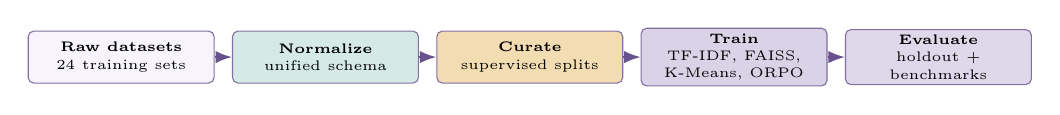
\begin{tikzpicture}[
  >=Latex,
  pipeline/.style={draw=lavenderDark!70, rounded corners=2pt, minimum height=0.66cm,
                   text width=2.22cm, align=center, inner sep=2pt,
                   font=\fontsize{5.4}{6.2}\selectfont\bfseries},
  pipearrow/.style={->, draw=lavenderDark!85, line width=0.65pt}]
  \node[pipeline, fill=lavenderLight!70] (raw) {Raw datasets\\\normalfont\fontsize{4.8}{5.4}\selectfont 24 training sets};
  \node[pipeline, fill=prismTeal!18, right=0.22cm of raw] (schema) {Normalize\\\normalfont\fontsize{4.8}{5.4}\selectfont unified schema};
  \node[pipeline, fill=prismGold!35, right=0.22cm of schema] (curate) {Curate\\\normalfont\fontsize{4.8}{5.4}\selectfont supervised splits};
  \node[pipeline, fill=prismBlue!28, right=0.22cm of curate] (train) {Train\\\normalfont\fontsize{4.8}{5.4}\selectfont TF-IDF, FAISS, K-Means, ORPO};
  \node[pipeline, fill=lavenderMedium!25, right=0.22cm of train] (eval) {Evaluate\\\normalfont\fontsize{4.8}{5.4}\selectfont holdout + benchmarks};
  \draw[pipearrow] (raw.east) -- (schema.west);
  \draw[pipearrow] (schema.east) -- (curate.west);
  \draw[pipearrow] (curate.east) -- (train.west);
  \draw[pipearrow] (train.east) -- (eval.west);
\end{tikzpicture}
\end{frame}


% The proposed methods frame is rendered above, before Model Responsibilities.
\iffalse
\begin{frame}[t]{06. Proposed Methods}
\vspace{0.02em}
\begin{center}
\parbox{0.95\linewidth}{%
\centering\fontsize{6.8}{8.6}\selectfont\color{lavenderDeep}%
\textbf{The proposed PrismSpace framework} transforms complex natural-language requests into reliable, verified outcomes through a four-stage orchestration pipeline. It routes user intent via contextual embeddings to select optimal model providers and specialist agents, plans execution using a dependency-aware Directed Acyclic Graph (DAG), executes sub-tasks through iterative ReAct loops with standardized MCP tools, and validates results using ORPO preference alignment and approval gates.%
}
\end{center}
\vspace{0.10em}
\begin{center}
\begin{tikzpicture}[
  >=Latex,
  method/.style={draw=lavenderDark!75, rounded corners=4pt, minimum height=1.48cm,
    text width=2.42cm, align=center, inner sep=4pt, line width=0.7pt,
    font=\fontsize{6.5}{7.7}\selectfont},
  methodarrow/.style={->, draw=lavenderDark!80, line width=0.9pt},
  loop/.style={draw=prismTeal!80!black, rounded corners=3pt, fill=white,
    minimum height=0.36cm, text width=0.74cm, align=center, inner sep=1pt,
    font=\fontsize{3.85}{4.35}\selectfont\bfseries}
]
  \node[method, fill=cInput!65] (route) {\textbf{1. Route}\\[0.18em]
    \normalfont\fontsize{5.7}{6.6}\selectfont Fuse context + embeddings\\ choose provider + agents};
  \node[method, fill=cPlanner!55, right=0.30cm of route] (dag) {\textbf{2. Plan}\\[0.18em]
    \normalfont\fontsize{5.7}{6.6}\selectfont Build a task DAG\\ run dependencies in order};
  \node[method, fill=cReact!60, draw=prismTeal!90!black, line width=1.05pt,
    text width=2.80cm, right=0.22cm of dag] (react) {\textbf{3. Execute}\\[0.08em]
    \normalfont\fontsize{5.6}{6.4}\selectfont
    \begin{tikzpicture}[baseline=-0.3ex, node distance=0.05cm]
      \node[loop, text width=0.74cm, fill=cReact!35] (obs) {Observe};
      \node[loop, text width=0.74cm, fill=cStage2!32, right=0.05cm of obs] (think) {Think};
      \node[loop, text width=0.74cm, fill=cTool!38, right=0.05cm of think] (act) {Act+MCP};
      \draw[methodarrow, draw=prismTeal!80!black, line width=0.55pt] (obs) -- (think);
      \draw[methodarrow, draw=prismTeal!80!black, line width=0.55pt] (think) -- (act);
      \draw[->, draw=prismTeal!80!black, line width=0.55pt] (act.south) .. controls +(0,-0.25) and +(0,-0.25) .. (obs.south);
    \end{tikzpicture}\\[-0.05em]
    \fontsize{5.1}{5.9}\selectfont Repeat until the sub-task is complete};
  \node[method, fill=cSafety!45, right=0.22cm of react] (verify) {\textbf{4. Verify}\\[0.18em]
    \normalfont\fontsize{5.7}{6.6}\selectfont ORPO + approval gate\\ save result in PrismDB};
  \draw[methodarrow] (route.east) -- (dag.west);
  \draw[methodarrow] (dag.east) -- (react.west);
  \draw[methodarrow] (react.east) -- (verify.west);
\end{tikzpicture}
\end{center}
\end{frame}
\fi

% =============================================================================
% SLIDE 7: END-TO-END SYSTEM FLOW (FIGURE 1.1) - removed from presentation
% =============================================================================
\iffalse
\section{System Flow}

\begin{frame}[t]{07. Overall End-to-End System Flow (Figure 1.1)}
\vspace{0.12cm}
\centering
\adjustbox{max height=0.86\textheight, max width=0.98\linewidth}{%
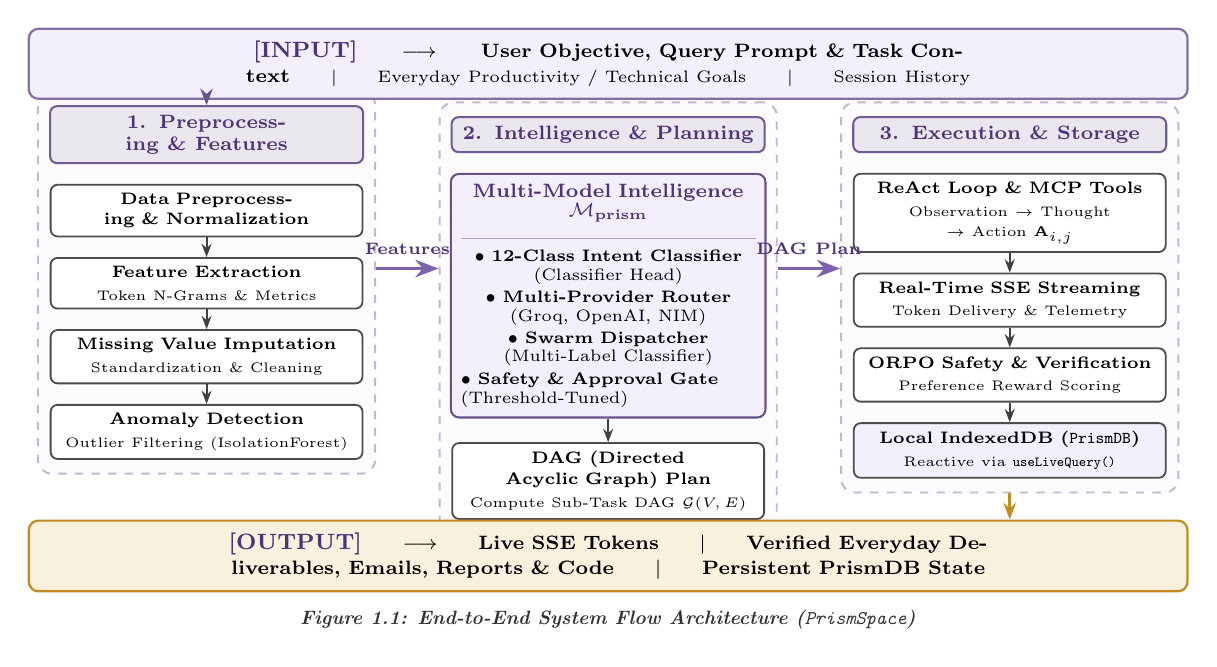
\begin{tikzpicture}[
    x=1cm, y=1cm,
    font=\sffamily,
    inout/.style={
        rectangle, rounded corners=3.5pt, line width=0.8pt,
        inner sep=4.5pt, align=center,
        font=\fontsize{7.2}{8.8}\selectfont
    },
    hdrbox/.style={
        rectangle, draw=lavenderDark!80, line width=0.75pt, fill=lavenderDark!12,
        rounded corners=2.5pt, inner sep=3.2pt, align=center,
        text width=3.75cm,
        font=\fontsize{6.8}{8.0}\selectfont\bfseries\color{lavenderDark}
    },
    stepbox/.style={
        rectangle, draw=black!70, line width=0.65pt, fill=white,
        rounded corners=2.5pt, inner sep=3.0pt, align=center,
        text width=3.75cm,
        font=\fontsize{6.2}{7.4}\selectfont
    },
    enginebox/.style={
        rectangle, draw=lavenderDark!85, line width=0.75pt, fill=lavenderLight,
        rounded corners=3pt, inner sep=3.5pt, align=left,
        text width=3.75cm,
        font=\fontsize{5.8}{7.0}\selectfont
    },
    stagebox/.style={
        rectangle, draw=lavenderDark!35, dashed, rounded corners=5pt, line width=0.7pt,
        fill=lavenderLight!25, inner xsep=4pt, inner ysep=5pt
    },
    flowarr/.style={
        -{Stealth[scale=0.75]}, line width=0.75pt, draw=black!75
    },
    transarr/.style={
        -{Stealth[scale=0.95]}, line width=1.3pt, draw=lavenderMedium
    }
]

    % 1. TOP: INPUT BAR
    \node [inout, fill=lavenderLight, draw=lavenderDark!70, text width=14.4cm] (input_node) at (0, 3.0) {
        \textbf{\fontsize{7.8}{9.2}\selectfont\color{lavenderDark}[INPUT]} $\;\longrightarrow\;$
        \textbf{User Objective, Query Prompt \& Task Context}
        {\fontsize{6.5}{7.8}\selectfont $\;\vert\;$ Everyday Productivity / Technical Goals $\;\vert\;$ Session History}
    };

    % 2. MIDDLE: 3-STAGE HORIZONTAL PIPELINE

    % --- STAGE 1: PREPROCESSING & FEATURES ---
    \node [hdrbox] (h1) at (-5.1, 2.1) {1. Preprocessing \& Features};
    \node [stepbox, below=0.25cm of h1] (s1_1) {\textbf{Data Preprocessing \& Normalization}};
    \node [stepbox, below=0.25cm of s1_1] (s1_2) {
        \textbf{Feature Extraction}\\[0.1em]
        {\fontsize{5.4}{6.4}\selectfont Token N-Grams \& Metrics}
    };
    \node [stepbox, below=0.25cm of s1_2] (s1_3) {
        \textbf{Missing Value Imputation}\\[0.1em]
        {\fontsize{5.4}{6.4}\selectfont Standardization \& Cleaning}
    };
    \node [stepbox, below=0.25cm of s1_3] (s1_4) {
        \textbf{Anomaly Detection}\\[0.1em]
        {\fontsize{5.4}{6.4}\selectfont Outlier Filtering (IsolationForest)}
    };

    \draw [flowarr] (s1_1) -- (s1_2);
    \draw [flowarr] (s1_2) -- (s1_3);
    \draw [flowarr] (s1_3) -- (s1_4);

    \begin{scope}[on background layer]
    \node [stagebox, fit=(h1) (s1_4)] (stage1) {};
    \end{scope}

    % --- STAGE 2: MULTI-MODEL INTELLIGENCE & DAG PLANNING ---
    \node [hdrbox] (h2) at (0, 2.1) {2. Intelligence \& Planning};
    \node [enginebox, below=0.25cm of h2] (s2_1) {
        \centering\textbf{\fontsize{6.8}{8.0}\selectfont\color{lavenderDark}Multi-Model Intelligence $\mathcal{M}_{\text{prism}}$}\\[0.15em]
        {\color{lavenderMedium!60}\rule{\linewidth}{0.4pt}}\\[0.2em]
        {\fontsize{5.6}{6.8}\selectfont
        $\bullet$ \textbf{12-Class Intent Classifier} (Classifier Head)\\[0.15em]
        $\bullet$ \textbf{Multi-Provider Router} (Groq, OpenAI, NIM)\\[0.15em]
        $\bullet$ \textbf{Swarm Dispatcher} (Multi-Label Classifier)\\[0.15em]
        $\bullet$ \textbf{Safety \& Approval Gate} (Threshold-Tuned)}
    };

    \node [stepbox, below=0.30cm of s2_1] (s2_2) {
        \textbf{DAG (Directed Acyclic Graph) Plan}\\[0.12em]
        {\fontsize{5.4}{6.4}\selectfont Compute Sub-Task DAG $\mathcal{G}(V, E)$}
    };

    \draw [flowarr] (s2_1) -- (s2_2);

    \begin{scope}[on background layer]
    \node [stagebox, fit=(h2) (s2_2)] (stage2) {};
    \end{scope}

    % --- STAGE 3: EXECUTION, STREAMING & PERSISTENCE ---
    \node [hdrbox] (h3) at (5.1, 2.1) {3. Execution \& Storage};
    \node [stepbox, below=0.25cm of h3] (s3_1) {
        \textbf{\fontsize{6.2}{7.3}\selectfont ReAct Loop \& MCP Tools}\\[0.1em]
        {\fontsize{5.4}{6.4}\selectfont Observation $\to$ Thought $\to$ Action $\mathbf{A}_{i,j}$}
    };
    \node [stepbox, below=0.25cm of s3_1] (s3_2) {
        \textbf{Real-Time SSE Streaming}\\[0.1em]
        {\fontsize{5.4}{6.4}\selectfont Token Delivery \& Telemetry}
    };
    \node [stepbox, below=0.25cm of s3_2] (s3_3) {
        \textbf{ORPO Safety \& Verification}\\[0.1em]
        {\fontsize{5.4}{6.4}\selectfont Preference Reward Scoring}
    };
    \node [stepbox, below=0.25cm of s3_3, fill=lavenderLight] (s3_4) {
        \textbf{Local IndexedDB (\texttt{PrismDB})}\\[0.1em]
        {\fontsize{5.4}{6.4}\selectfont Reactive via \texttt{useLiveQuery()}}
    };

    \draw [flowarr] (s3_1) -- (s3_2);
    \draw [flowarr] (s3_2) -- (s3_3);
    \draw [flowarr] (s3_3) -- (s3_4);

    \begin{scope}[on background layer]
    \node [stagebox, fit=(h3) (s3_4)] (stage3) {};
    \end{scope}

    % Transition arrows between stages
    \draw [transarr] ($(stage1.east |- 0, 0.4)$) -- 
        node[above=1pt, font=\fontsize{6.0}{7.0}\selectfont\bfseries\color{lavenderDark}]{Features} ($(stage2.west |- 0, 0.4)$);

    \draw [transarr] ($(stage2.east |- 0, 0.4)$) -- 
        node[above=1pt, font=\fontsize{6.0}{7.0}\selectfont\bfseries\color{lavenderDark}]{DAG Plan} ($(stage3.west |- 0, 0.4)$);

    \draw [flowarr, line width=1.1pt, draw=lavenderDark!85] (input_node.south -| h1.north) -- (h1.north);

    % 3. BOTTOM: OUTPUT BAR
    \node [inout, fill=prismGold!15, draw=prismGold!90!black, text width=14.4cm, below=0.45cm of $(stage1.south)!0.5!(stage3.south)$] (output_node) {
        \textbf{\fontsize{7.8}{9.2}\selectfont\color{lavenderDark}[OUTPUT]} $\;\longrightarrow\;$
        \textbf{Live SSE Tokens} $\;\vert\;$
        \textbf{Verified Everyday Deliverables, Emails, Reports \& Code} $\;\vert\;$
        \textbf{Persistent PrismDB State}
    };

    \draw [flowarr, line width=1.1pt, draw=prismGold!90!black] (stage3.south -| h3.south) -- (output_node.north -| h3.south);

    % Caption
    \node [font=\fontsize{7.2}{8.5}\selectfont\bfseries\color{black!80}, below=0.10cm of output_node] {
        \textit{Figure 1.1: End-to-End System Flow Architecture (\texttt{PrismSpace})}
    };

\end{tikzpicture}%
}
\end{frame}
\fi

% =============================================================================
% SLIDE 8: SIMPLIFIED FLOW STAGES 1, 2, & 3
% =============================================================================
\begin{frame}[t]{11. How the System Works: From Request to Result}
\vspace{-0.55em}
\begin{columns}[T]
\begin{column}{0.32\textwidth}
  \begin{tcolorbox}[
    enhanced, arc=3pt, colframe=lavenderDark, colback=white,
    title={\scriptsize\bfseries Stage 1: Ingestion \& Features},
    boxrule=0.55pt, left=3.5pt, right=3.5pt, top=1.0pt, bottom=1.0pt
  ]
  \fontsize{5.8}{6.8}\selectfont
  \begin{itemize}\setlength{\itemsep}{0.8pt}
    \item \textbf{Capture request:} Parse user input (text/voice/API).
    \item \textbf{Clean \& normalize:} Remove noise, handle missing data with NLP preprocessing.
    \item \textbf{Extract features:} Tokenize into semantic embeddings using transformer models.
  \end{itemize}
  \end{tcolorbox}
\end{column}

\begin{column}{0.34\textwidth}
  \begin{tcolorbox}[
    enhanced, arc=3pt, colframe=prismTeal, colback=white,
    title={\scriptsize\bfseries Stage 2: Intelligence \& DAG},
    boxrule=0.55pt, left=3.5pt, right=3.5pt, top=1.0pt, bottom=1.0pt
  ]
  \fontsize{5.8}{6.8}\selectfont
  \begin{itemize}\setlength{\itemsep}{0.8pt}
    \item \textbf{Classify intent:} ML classifier identifies task type from 12 categories (99.6\% accuracy).
    \item \textbf{Choose agents \& models:} Route sub-tasks to specialized LLM agents.
    \item \textbf{Build the DAG:} Create dependency graph ensuring safe execution order.
  \end{itemize}
  \end{tcolorbox}
\end{column}

\begin{column}{0.32\textwidth}
  \begin{tcolorbox}[
    enhanced, arc=3pt, colframe=lavenderMedium, colback=white,
    title={\scriptsize\bfseries Stage 3: Execution \& Storage},
    boxrule=0.55pt, left=3.5pt, right=3.5pt, top=1.0pt, bottom=1.0pt
  ]
  \fontsize{5.8}{6.8}\selectfont
  \begin{itemize}\setlength{\itemsep}{0.8pt}
    \item \textbf{Execute:} Run up to 3 parallel tasks using Model Context Protocol (MCP) tools.
    \item \textbf{Track progress:} Real-time telemetry, node state transitions, and execution logs.
    \item \textbf{Verify \& store:} ORPO quality check, persist results to PrismDB.
  \end{itemize}
  \end{tcolorbox}
\end{column}
\end{columns}

\vspace{-0.65em}
\begin{tcolorbox}[
  enhanced, arc=3pt, colframe=prismTeal!85!black, colback=white, boxrule=0.65pt,
  left=3.5pt, right=3.5pt, top=1.0pt, bottom=1.0pt,
  title={\scriptsize\bfseries Building \& Executing the Task Graph $\mathcal{G}(V, E)$}
]
\centering
\adjustbox{max width=0.99\linewidth, max height=0.485\textheight, keepaspectratio}{%
\begin{tikzpicture}[
  dagstep/.style={rectangle, rounded corners=2pt, minimum height=0.38cm,
    text width=2.95cm, align=center, draw=lavenderDark!55, fill=lavenderLight!55,
    font=\fontsize{4.8}{5.6}\selectfont\bfseries},
  dagarrow/.style={-{Stealth[scale=0.55]}, line width=0.7pt, draw=prismTeal!85!black}
]
  % Row 1: 4-Step Pipeline Across Top
  \node[dagstep] (s1) at (-5.25, 0.28) {1. User Goal Prompt\\\normalfont\fontsize{4.2}{4.8}\selectfont ``Analyze news+CSV, email summary''};
  \node[dagstep] (s2) at (-1.75, 0.28) {2. Split into Vertices $V$\\\normalfont\fontsize{4.2}{4.8}\selectfont Modular async tasks $A, B, C, D$};
  \node[dagstep] (s3) at (1.75, 0.28) {3. Connect Edges $E$\\\normalfont\fontsize{4.2}{4.8}\selectfont Map output return $\to$ input args};
  \node[dagstep] (s4) at (5.25, 0.28) {4. Topological Run\\\normalfont\fontsize{4.2}{4.8}\selectfont Run in-degree $=0 \implies$ join barrier};
  \draw[dagarrow] (s1) -- (s2);
  \draw[dagarrow] (s2) -- (s3);
  \draw[dagarrow] (s3) -- (s4);

  % Row 2 Left: Computer Science Concept Walkthrough
  \node[rectangle, rounded corners=2.5pt, draw=lavenderMedium!60, fill=lavenderLight!30,
        line width=0.55pt, text width=7.4cm, inner sep=2.4pt, align=left, anchor=north] at (-3.45, -0.06) {%
    \fontsize{4.8}{5.8}\selectfont\textbf{\color{lavenderDark}\faCode\ Computer Science Explanation (By Concrete Example):}\\[0.8pt]
    \fontsize{4.0}{4.8}\selectfont
    $\bullet$\enspace\textbf{Vertices ($V$) = Sub-Task Functions (Async Call Units):}\\
    \enspace\enspace Node $A$: \texttt{news = await SearchWeb("Tesla news")} \hfill \textit{[Researcher]}\\
    \enspace\enspace Node $B$: \texttt{data = await FetchCSV("metrics.csv")} \hfill \textit{[Data Agent]}\\
    \enspace\enspace Node $C$: \texttt{rep = await Synthesize(news, data)} \hfill \textit{[Writer Agent]}\\
    \enspace\enspace Node $D$: \texttt{await SendEmail(to="lead", body=rep)} \hfill \textit{[Email Tool]}\\[0.6pt]
    $\bullet$\enspace\textbf{Edges ($E$) = Data Pipes \& Synchronization Barriers:}\\
    \enspace\enspace Edge $\langle A, C\rangle$ pipes return value \texttt{news}; edge $\langle B, C\rangle$ pipes \texttt{data}.\\
    \enspace\enspace Barrier: task $C$ blocks until both promises $A$ \& $B$ resolve.\\[0.6pt]
    $\bullet$\enspace\textbf{Connection Basis (Input $\leftarrow$ Output Matching):}\\
    \enspace\enspace Function $C$ links to $A$ \& $B$ because $C$'s parameters require their outputs.\\
    \enspace\enspace $A$ and $B$ share no edge because neither depends on the other's data.\\[0.6pt]
    $\bullet$\enspace\textbf{Execution Schedule (Topological Concurrency):}\\
    \enspace\enspace Tasks with $\text{in-degree} = 0$ ($A, B$) execute \textbf{concurrently in parallel}.\\
    \enspace\enspace When $A$ \& $B$ complete, $C$'s in-degree drops to $0 \implies C$ runs $\implies D$ runs.%
  };

  % Row 2 Right: Visual Data-Flow Graph
  \node[rectangle, rounded corners=2.5pt, draw=prismTeal!60, fill=white,
        line width=0.55pt, text width=5.6cm, inner sep=2.5pt, align=center, anchor=north] at (3.65, -0.06) {%
    \fontsize{4.6}{5.5}\selectfont\textbf{\color{prismTeal!90!black}\faProjectDiagram\ Visual Data-Flow Graph \& Execution Order}\\[1.2pt]
    \begin{tikzpicture}[
      cnode/.style={rectangle, rounded corners=2pt, draw=prismTeal!90!black, fill=prismMint,
        line width=0.55pt, minimum height=0.34cm, inner sep=1.8pt, align=center,
        font=\fontsize{3.8}{4.5}\selectfont},
      earr/.style={-{Stealth[scale=0.48]}, line width=0.60pt, draw=prismTeal!85!black}
    ]
      % Nodes
      \node[cnode, text width=1.45cm] (na) at (-1.95, 0.36) {\textbf{Node A}: \texttt{SearchWeb}\\ \fontsize{3.1}{3.6}\selectfont\color{prismDark}in-degree $=0$ (Parallel)};
      \node[cnode, text width=1.45cm] (nb) at (-1.95, -0.36) {\textbf{Node B}: \texttt{FetchCSV}\\ \fontsize{3.1}{3.6}\selectfont\color{prismDark}in-degree $=0$ (Parallel)};

      \node[cnode, text width=1.50cm] (nc) at (0.05, 0) {\textbf{Node C}: \texttt{Synthesize}\\ \fontsize{3.1}{3.6}\selectfont\color{prismDark}Barrier: awaits $A$ \& $B$};

      \node[cnode, text width=1.40cm] (nd) at (1.95, 0) {\textbf{Node D}: \texttt{SendEmail}\\ \fontsize{3.1}{3.6}\selectfont\color{prismDark}Final Deliverable};

      % Edges with data flow labels
      \draw[earr] (na.east) -- node[above, sloped, font=\fontsize{3.1}{3.6}\selectfont\bfseries, text=lavenderDark, fill=white, inner sep=0.7pt] {\texttt{news}} (nc.west);
      \draw[earr] (nb.east) -- node[below, sloped, font=\fontsize{3.1}{3.6}\selectfont\bfseries, text=lavenderDark, fill=white, inner sep=0.7pt] {\texttt{data}} (nc.west);
      \draw[earr] (nc.east) -- node[above, font=\fontsize{3.1}{3.6}\selectfont\bfseries, text=lavenderDark, fill=white, inner sep=0.7pt] {\texttt{rep}} (nd.west);
    \end{tikzpicture}\\[1.0pt]
    \fontsize{3.7}{4.4}\selectfont
    \textbf{Parallel Thread 1:} Worker 1 executes Node A $\to$ returns \texttt{news}\\[0.3pt]
    \textbf{Parallel Thread 2:} Worker 2 executes Node B $\to$ returns \texttt{data}\\[0.3pt]
    \textbf{Join Barrier:} Node C consumes \texttt{news} + \texttt{data} $\to$ outputs \texttt{rep}\\[0.3pt]
    \textbf{Serial Finish:} Node D consumes \texttt{rep} $\to$ sends email
  };

\end{tikzpicture}%
}
\end{tcolorbox}
\end{frame}

% =============================================================================
% SLIDE 9: SYSTEM ARCHITECTURE (FIGURE 1.2)
% =============================================================================
\section{System Architecture}

\begin{frame}[t]{12. PrismSpace System Architecture \& Multi-Model Swarm Workflow (Figure 1.2)}
\vspace{-0.30em}
\centering
\adjustbox{max width=0.99\linewidth, max height=0.88\textheight, keepaspectratio}{%
\begin{tikzpicture}[
  x=1cm, y=1cm,
  every node/.style={align=center},
  group/.style={draw=lavenderMedium!60, dashed, line width=0.75pt,
    fill=lavenderLight!20, rounded corners=6pt},
  grouptitle/.style={fill=lavenderDark, text=white, font=\fontsize{5.5}{6.5}\selectfont\bfseries,
    rounded corners=2.5pt, inner xsep=6pt, inner ysep=2.2pt},
  colbox/.style={rectangle, rounded corners=3pt, line width=0.65pt,
    minimum height=0.60cm, inner ysep=2.5pt, inner xsep=4pt,
    font=\fontsize{5.2}{6.2}\selectfont\bfseries},
  modelbox/.style={rectangle, rounded corners=2.5pt, line width=0.65pt,
    draw=lavenderDark!85, fill=white,
    minimum height=0.60cm, inner ysep=2.2pt, inner xsep=3pt,
    font=\fontsize{4.8}{5.8}\selectfont},
  arrow/.style={
    -{Stealth[scale=0.75]}, line width=0.75pt, draw=lavenderDark!85
  },
  modelarrow/.style={
    -{Stealth[scale=0.65]}, line width=0.65pt, draw=lavenderDark!75
  },
  badge/.style={
    fill=white, draw=lavenderMedium!80, rounded corners=2pt, line width=0.45pt,
    inner xsep=3.5pt, inner ysep=1.6pt, font=\fontsize{4.2}{5.2}\selectfont\bfseries
  }
]

  % =========================================================================
  % COLUMN 1: PRESENTATION & API GATEWAY
  % Center: 1.38, width: 2.65cm, height: 6.30cm, Center Y = 3.30
  % Group span: [0.055, 2.705]
  % =========================================================================
  \node[group, minimum width=2.65cm, minimum height=6.30cm] (g1) at (1.38, 3.30) {};
  \node[grouptitle, anchor=west] at (0.15, 6.45) {1. Presentation \& API Gateway};

  \node[colbox, text width=2.45cm, fill=cInput, draw=prismSlate!70] (g1_user) at (1.38, 5.60) {%
    \faUser\ \textbf{User Objective Ingestion}\\[1.5pt]
    {\fontsize{4.1}{5.0}\selectfont Natural Language Prompt\\[0.5pt]Scope Bounds ($K \le 3$)}%
  };

  \node[colbox, text width=2.45cm, fill=cStem, draw=prismIndigo!70] (g1_ui) at (1.38, 4.20) {%
    \faDesktop\ \textbf{Next.js 15 Client UI}\\[1.5pt]
    {\fontsize{4.1}{5.0}\selectfont React 19 Dashboard\\[0.5pt]Swarm Visualizer}%
  };

  \node[colbox, text width=2.45cm, fill=cPlanner, draw=prismBlue!80] (g1_gw) at (1.38, 2.75) {%
    \faServer\ \textbf{FastAPI Hive Gateway}\\[1.5pt]
    {\fontsize{4.1}{5.0}\selectfont REST API $\cdot$ Tool Registry\\[0.5pt]Real-Time Token Streaming}%
  };

  \node[colbox, text width=2.45cm, fill=cInput!60, draw=prismSlate!60] (g1_telemetry) at (1.38, 1.25) {%
    \faChartBar\ \textbf{Telemetry \& Observability}\\[1.5pt]
    {\fontsize{4.1}{5.0}\selectfont Event Logging\\[0.5pt]Metrics Monitoring}%
  };

  \draw[arrow] (g1_user) -- (g1_ui);
  \draw[arrow] (g1_ui) -- (g1_gw);
  \draw[arrow] (g1_gw) -- (g1_telemetry);

  % =========================================================================
  % COLUMN 2: ML ROUTING & HYBRID RETRIEVAL
  % Center: 5.95, width: 4.60cm, height: 6.30cm, Center Y = 3.30
  % Group span: [3.65, 8.25]
  % =========================================================================
  \node[group, minimum width=4.60cm, minimum height=6.30cm] (g2) at (5.95, 3.30) {};
  \node[grouptitle, anchor=west] at (3.75, 6.45) {2. ML Routing \& Hybrid Retrieval};

  \node[colbox, text width=4.30cm, fill=cDispatch, draw=prismBlue!85] (g2_feat) at (5.95, 5.60) {%
    \faCogs\ \textbf{Feature Extraction \& Vectorization}\\[1.5pt]
    {\fontsize{4.1}{5.0}\selectfont Convert text to numbers + Statistical word patterns\\[0.5pt]Multi-Source Training Corpora}%
  };

  % 2x2 Model Grid
  \node[modelbox, text width=2.00cm, fill=cHead!45] (m_intent) at (4.80, 4.35) {%
    \faBrain\ \textbf{Intent Classifier}\\[1.5pt]
    {\fontsize{4.0}{4.8}\selectfont 12 Calibrated Domains}\\[0.5pt]
    {\fontsize{3.6}{4.4}\selectfont\itshape (code, data, web, etc.)}%
  };
  \node[modelbox, text width=2.00cm, fill=cStage1!45] (m_agent) at (7.10, 4.35) {%
    \faUsers\ \textbf{Swarm Agent Router}\\[1.5pt]
    {\fontsize{4.0}{4.8}\selectfont Specialist Dispatch ($K \le 3$)}%
  };
  \node[modelbox, text width=2.00cm, fill=cStage4!45] (m_model) at (4.80, 3.05) {%
    \faRandom\ \textbf{Provider Router}\\[1.5pt]
    {\fontsize{4.0}{4.8}\selectfont Groq, OpenAI, Anthropic, NIM}%
  };
  \node[modelbox, text width=2.00cm, fill=cTool!45] (m_cost) at (7.10, 3.05) {%
    \faChartLine\ \textbf{Cost \& Latency}\\[1.5pt]
    {\fontsize{4.0}{4.8}\selectfont Predictive Execution Bounds}%
  };

  \node[colbox, text width=4.30cm, fill=cMemory, draw=purple!60!black] (g2_rank) at (5.95, 1.35) {%
    \faSearch\ \textbf{Hybrid Retrieval Ranker}\\[1.5pt]
    {\fontsize{4.1}{5.0}\selectfont Dense Vector Embedding Search + Keyword Relevance Match\\[0.5pt]
    Context Window Selection $\cdot$ Specialist Knowledge Bases}%
  };

  % Connectors inside Col 2
  \draw[modelarrow] (g2_feat.south) -- (5.95, 5.00) -| (m_intent.north);
  \draw[modelarrow] (g2_feat.south) -- (5.95, 5.00) -| (m_agent.north);
  \draw[modelarrow] (m_intent.south) -- (m_model.north);
  \draw[modelarrow] (m_agent.south) -- (m_cost.north);
  \draw[modelarrow] (m_model.south) -- (4.80, 2.25) -- (5.95, 2.25) -- (g2_rank.north);
  \draw[modelarrow] (m_cost.south) -- (7.10, 2.25) -- (5.95, 2.25);

  % =========================================================================
  % COLUMN 3: SWARM DAG, SEPARATE AGENT BOXES, SAFETY & SEPARATE OUTPUTS
  % Center: 11.90, width: 5.80cm, height: 6.30cm, Center Y = 3.30
  % Group span: [9.00, 14.80]
  % =========================================================================
  \node[group, minimum width=5.80cm, minimum height=6.30cm] (g3) at (11.90, 3.30) {};
  \node[grouptitle, anchor=west] at (9.10, 6.45) {3. Swarm DAG, Specialist Agents, Safety \& Outputs};

  % 1. DAG Task Planner
  \node[colbox, text width=5.40cm, fill=cReact, draw=prismTeal!90] (g3_dag) at (11.90, 5.60) {%
    \faProjectDiagram\ \textbf{DAG Task Planner $\mathcal{G}(V, E)$}\\[1.5pt]
    {\fontsize{4.1}{5.0}\selectfont Workflow DAG Generation \& Scheduling $\cdot$ Success Probability Forecaster}%
  };

  % 2. THREE SEPARATE AGENT BOXES (Side-by-Side with clear roles and tools!)
  % Centers: 9.95, 11.90, 13.85 (width: 1.65cm each, height: 1.35cm, Y = 4.15)
  \node[colbox, text width=1.55cm, minimum height=1.35cm, fill=cTool!80, draw=prismGold!95!black, inner sep=2.5pt] (ag_coder) at (9.95, 4.15) {%
    \textbf{\fontsize{4.9}{5.9}\selectfont\color{prismTeal!90!black}\faCode\ Coder Agent}\\[2.5pt]
    {\fontsize{3.7}{4.5}\selectfont Edits source code,\\[1pt]CLI terminal tools,\\[1pt]syntax debugging}%
  };

  \node[colbox, text width=1.55cm, minimum height=1.35cm, fill=cTool!80, draw=prismGold!95!black, inner sep=2.5pt] (ag_assist) at (11.90, 4.15) {%
    \textbf{\fontsize{4.9}{5.9}\selectfont\color{prismBlue}\faSearch\ Assistant Agent}\\[2.5pt]
    {\fontsize{3.7}{4.5}\selectfont Web research,\\[1pt]Gmail \& Drive tools,\\[1pt]context synthesis}%
  };

  \node[colbox, text width=1.55cm, minimum height=1.35cm, fill=cTool!80, draw=prismGold!95!black, inner sep=2.5pt] (ag_val) at (13.85, 4.15) {%
    \textbf{\fontsize{4.9}{5.9}\selectfont\color{purple!75!black}\faClipboardCheck\ Validator Agent}\\[2.5pt]
    {\fontsize{3.7}{4.5}\selectfont Output reviews,\\[1pt]test assertion suites,\\[1pt]safety policy checks}%
  };

  % 3. Safety Triad & HITL Gate
  \node[colbox, text width=5.40cm, fill=cSafety!50, draw=red!70!black] (g3_safety) at (11.90, 2.75) {%
    \faLock\ \textbf{Safety Triad \& HITL Checkpoint Gate}\\[1.5pt]
    {\fontsize{4.1}{5.0}\selectfont Approval Risk Scorer $\cdot$ Anomaly Detector $\cdot$ ORPO Alignment Scorer}%
  };

  % 4. Approval Badge
  \node[badge, draw=green!60!black, text=green!55!black] (b_app) at (11.90, 2.05) {\faCheck\ Approved: Commit Deliverables};

  % 5. FOUR SEPARATE OUTPUT BOXES (2x2 Grid with generous central spacing!)
  % Row 1 at Y = 1.35, Row 2 at Y = 0.55
  % Left Col: 10.35, Right Col: 13.45 (width: 2.35cm each, height: 0.65cm)
  \node[colbox, text width=2.25cm, minimum height=0.62cm, fill=cDeliverable!95, draw=prismTeal!80!black, inner sep=2.0pt] (out_gmail) at (10.35, 1.35) {%
    \textbf{\fontsize{4.8}{5.8}\selectfont\color{red!70!black}\faEnvelope\ Gmail Actions}\\[1.5pt]
    {\fontsize{3.7}{4.5}\selectfont Sent emails, replies \& drafts}%
  };

  \node[colbox, text width=2.25cm, minimum height=0.62cm, fill=cDeliverable!95, draw=prismTeal!80!black, inner sep=2.0pt] (out_drive) at (13.45, 1.35) {%
    \textbf{\fontsize{4.8}{5.8}\selectfont\color{prismBlue!90!black}\faGoogleDrive\ Google Drive Sync}\\[1.5pt]
    {\fontsize{3.7}{4.5}\selectfont Synced docs \& spreadsheets}%
  };

  \node[colbox, text width=2.25cm, minimum height=0.62cm, fill=cDeliverable!95, draw=prismTeal!80!black, inner sep=2.0pt] (out_code) at (10.35, 0.55) {%
    \textbf{\fontsize{4.8}{5.8}\selectfont\color{prismTeal!90!black}\faFileCode\ Code \& Terminal}\\[1.5pt]
    {\fontsize{3.7}{4.5}\selectfont Source patches \& CLI builds}%
  };

  \node[colbox, text width=2.25cm, minimum height=0.62cm, fill=cDeliverable!95, draw=prismTeal!80!black, inner sep=2.0pt] (out_db) at (13.45, 0.55) {%
    \textbf{\fontsize{4.8}{5.8}\selectfont\color{purple!75!black}\faDatabase\ PrismDB \& Live UI}\\[1.5pt]
    {\fontsize{3.7}{4.5}\selectfont 17 Dexie tables \& token stream}%
  };

  % Connectors inside Col 3
  % DAG Planner -> 3 Agents
  \draw[arrow] (g3_dag.south) -- (11.90, 5.00) -| (ag_coder.north);
  \draw[arrow] (g3_dag.south) -- (ag_assist.north);
  \draw[arrow] (g3_dag.south) -- (11.90, 5.00) -| (ag_val.north);

  % 3 Agents -> Safety Gate
  \draw[arrow] (ag_coder.south) |- (11.90, 3.30) -- (g3_safety.north);
  \draw[arrow] (ag_assist.south) -- (g3_safety.north);
  \draw[arrow] (ag_val.south)   |- (11.90, 3.30) -- (g3_safety.north);

  % Safety Gate -> Commit Badge -> 4 Output Boxes via clean central bus
  \draw[arrow, draw=green!60!black, line width=0.75pt] (g3_safety.south) -- (b_app.north);
  \draw[-, draw=green!60!black, line width=0.75pt] (b_app.south) -- (11.90, 0.55);
  \draw[arrow, draw=green!60!black, line width=0.65pt] (11.90, 1.35) -- (out_gmail.east);
  \draw[arrow, draw=green!60!black, line width=0.65pt] (11.90, 1.35) -- (out_drive.west);
  \draw[arrow, draw=green!60!black, line width=0.65pt] (11.90, 0.55) -- (out_code.east);
  \draw[arrow, draw=green!60!black, line width=0.65pt] (11.90, 0.55) -- (out_db.west);

  % Re-Plan / Feedback Loop (Right margin at x=15.40 - ample clearance from ag_val at 14.675!)
  \draw[arrow, draw=red!75!black, line width=0.75pt] (g3_safety.east) -- (15.40, 2.75) -- (15.40, 5.60) -- (g3_dag.east);
  \node[badge, draw=red!75!black, text=red!75!black] at (15.40, 4.15) {\faTimes\ Re-Plan};

  % =========================================================================
  % INTER-COLUMN PIPELINE ROUTING
  % =========================================================================
  % Gateway -> Feature Extraction (Channel 1: mid = 3.14)
  \draw[arrow, draw=lavenderDark!90, line width=0.75pt] (g1_gw.east) -- (3.14, 2.75) -- (3.14, 5.60) -- (g2_feat.west);
  \node[badge, text=lavenderDark] at (3.14, 3.45) {REST / Stream};

  % Channel 2: Routing Spec -> DAG Planner (mid = 8.62)
  \draw[arrow, draw=lavenderDark!90, line width=0.75pt] (m_agent.east) -- (8.62, 4.35) -- (8.62, 5.60) -- (g3_dag.west);
  \node[badge, text=lavenderDark] at (8.62, 5.05) {Routing};

  % Channel 2: Context -> Agents (mid = 8.62)
  \draw[arrow, draw=lavenderDark!90, line width=0.75pt] (g2_rank.east) -- (8.62, 1.35) -- (8.62, 4.15) -- (ag_coder.west);
  \node[badge, text=lavenderDark] at (8.62, 2.75) {Context};

\end{tikzpicture}%
}
\end{frame}

% % =============================================================================
% SLIDE 13: FLOWCHART DIAGRAM (Multi-Agent Communication Flow)
% =============================================================================
\begin{frame}[t]{13. Flowchart: Multi-Agent Execution Flow (Figure 1.3)}
\vspace{-0.30em}
\centering
\adjustbox{max width=0.99\linewidth, max height=0.88\textheight, keepaspectratio}{%
\begin{tikzpicture}[
  x=1cm, y=1cm,
  font=\sffamily,
  % Node Styles
  startend/.style={
    ellipse, draw=green!60!black, fill=green!45!black, text=white,
    line width=0.85pt, inner sep=2.5pt, font=\fontsize{6.0}{7.0}\selectfont\bfseries,
    minimum width=1.45cm, minimum height=0.50cm, drop shadow={opacity=0.12, shadow xshift=0.5pt, shadow yshift=-0.5pt}
  },
  userbox/.style={
    rectangle, rounded corners=3.5pt,
    draw=cyan!70!black, fill=cyan!14, text=black,
    line width=0.85pt, inner sep=3.5pt, font=\fontsize{6.2}{7.2}\selectfont\bfseries,
    minimum height=0.68cm, align=center, drop shadow={opacity=0.10, shadow xshift=0.5pt, shadow yshift=-0.5pt}
  },
  agentbox/.style={
    rectangle, rounded corners=3.5pt,
    draw=orange!80!black, fill=orange!16, text=black,
    line width=0.85pt, inner sep=3.5pt, font=\fontsize{6.2}{7.2}\selectfont\bfseries,
    minimum height=0.68cm, align=center, drop shadow={opacity=0.10, shadow xshift=0.5pt, shadow yshift=-0.5pt}
  },
  decision/.style={
    diamond, aspect=1.55,
    draw=lavenderDark!90, fill=lavenderLight, text=lavenderDark,
    line width=0.85pt, inner sep=1.5pt, font=\fontsize{5.6}{6.6}\selectfont\bfseries,
    minimum width=1.85cm, align=center, drop shadow={opacity=0.10, shadow xshift=0.5pt, shadow yshift=-0.5pt}
  },
  processbox/.style={
    rectangle, rounded corners=3.5pt,
    draw=prismTeal!85!black, fill=prismMint, text=black,
    line width=0.85pt, inner sep=3.5pt, font=\fontsize{6.2}{7.2}\selectfont\bfseries,
    minimum height=0.68cm, align=center, drop shadow={opacity=0.10, shadow xshift=0.5pt, shadow yshift=-0.5pt}
  },
  toolbox/.style={
    rectangle, rounded corners=3pt,
    draw=prismGold!85!black, fill=prismGold!14, text=black,
    line width=0.75pt, inner sep=2.5pt, font=\fontsize{5.0}{6.0}\selectfont,
    minimum height=0.56cm, align=center
  },
  deliverbox/.style={
    rectangle, rounded corners=3.5pt,
    draw=green!65!black, fill=green!12, text=black,
    line width=0.85pt, inner sep=3.0pt, font=\fontsize{6.0}{7.0}\selectfont\bfseries,
    minimum height=0.68cm, align=center, drop shadow={opacity=0.10, shadow xshift=0.5pt, shadow yshift=-0.5pt}
  },
  fixbox/.style={
    rectangle, rounded corners=3.5pt,
    draw=red!75!black, fill=red!10, text=black,
    line width=0.85pt, inner sep=3.0pt, font=\fontsize{6.0}{7.0}\selectfont\bfseries,
    minimum height=0.68cm, align=center, drop shadow={opacity=0.10, shadow xshift=0.5pt, shadow yshift=-0.5pt}
  },
  stagehdr/.style={
    font=\fontsize{5.4}{6.4}\selectfont\bfseries, text=white,
    rounded corners=2.5pt, inner xsep=4.5pt, inner ysep=2.0pt
  },
  arr/.style={-{Stealth[scale=0.75]}, line width=0.90pt, draw=black!75},
  redarr/.style={-{Stealth[scale=0.75]}, line width=0.90pt, draw=red!75!black},
  dasharr/.style={-{Stealth[scale=0.65]}, line width=0.75pt, draw=lavenderMedium, dashed},
  stagebox/.style={
    rectangle, rounded corners=5pt, line width=0.6pt
  }
]

% =========================================================================
% LEFT / CENTER WORKFLOW (Center X = 5.80)
% =========================================================================

% --- STAGE 1: USER OBJECTIVE & INTENT INGESTION (Y: 5.30 to 8.45) ---
\node[startend] (start) at (5.80, 8.00) {\faPlay\ START};

\node[userbox, text width=4.3cm] (user) at (5.80, 7.05) {
  \faUser\ \textbf{1. User Objective}\\[-0.05em]
  {\fontsize{5.2}{6.2}\selectfont\normalfont\color{black!80} ``Build auth module with SQL DB''}
};

\node[agentbox, text width=4.3cm] (classifier) at (5.80, 5.95) {
  \faBrain\ \textbf{2. Intent Classifier \& Router}\\[-0.05em]
  {\fontsize{5.0}{6.0}\selectfont\normalfont\color{black!80} Identifies domain (1 of 12 classes) \& provider}\\[-0.05em]
  {\fontsize{4.6}{5.6}\selectfont\itshape\color{orange!90!black} (OpenAI, Claude, Gemini, Groq, NVIDIA)}
};

\draw[arr] (start) -- (user);
\draw[arr] (user) -- (classifier);

% --- STAGE 2: EXECUTION DAG PLANNER & DISPATCH (Y: 3.75 to 5.20) ---
\node[processbox, text width=4.00cm] (planner) at (5.80, 4.45) {
  \faProjectDiagram\ \textbf{DAG Task Planner}\\[-0.05em]
  {\fontsize{4.8}{5.8}\selectfont\normalfont Compiles task DAG $\mathcal{G}(V, E)$ from objective}
};

% Annotation to the right of planner node (clear corridor, zero collision)
\node[rectangle, rounded corners=3pt, fill=cyan!10, draw=cyan!60, line width=0.5pt,
      text width=2.45cm, align=left, inner sep=2.8pt] at (9.48, 4.45) {
  \fontsize{4.2}{5.2}\selectfont
  \textbf{\color{prismTeal!90!black}\faSitemap\ Swarm Bounding:}\\
  $\bullet$\enspace Dispatches $K \le 3$ workers\\
  $\bullet$\enspace Dependency-aware scheduling
};

\draw[arr] (classifier) -- (planner);

% --- STAGE 3: WORKER SWARM & MCP TOOL SERVERS (Y: 0.90 to 3.65) ---
% Worker A: Research & Context (X = 2.05)
\node[agentbox, text width=2.30cm] (workera) at (2.05, 2.50) {
  \faSearch\ \textbf{Agent-A (Research)}\\[-0.05em]
  {\fontsize{4.8}{5.8}\selectfont\normalfont Context \& spec analysis}
};
\node[toolbox, text width=2.30cm] (toola) at (2.05, 1.52) {
  \textbf{\faGlobe\ Browser MCP / Docs:}\\[-0.05em]
  {\fontsize{4.6}{5.5}\selectfont $\bullet$ Web scraper \quad $\bullet$ Specs}
};
\draw[dasharr] (workera) -- node[right, font=\fontsize{4.0}{4.8}\selectfont\color{lavenderDark}]{ReAct} (toola);

% Worker B: Code & Terminal (X = 5.80)
\node[agentbox, text width=2.30cm] (workerb) at (5.80, 2.50) {
  \faCode\ \textbf{Agent-B (Coding)}\\[-0.05em]
  {\fontsize{4.7}{5.7}\selectfont\normalfont Logic \& API implementation}
};
\node[toolbox, text width=2.30cm] (toolb) at (5.80, 1.52) {
  \textbf{\faTerminal\ Terminal / FS MCP:}\\[-0.05em]
  {\fontsize{4.6}{5.5}\selectfont $\bullet$ Shell CLI \quad $\bullet$ File edit}
};
\draw[dasharr] (workerb) -- node[right, font=\fontsize{4.0}{4.8}\selectfont\color{lavenderDark}]{ReAct} (toolb);

% Worker C: Validation & Database (X = 9.55)
\node[agentbox, text width=2.30cm] (workerc) at (9.55, 2.50) {
  \faCheckCircle\ \textbf{Agent-C (Validation)}\\[-0.05em]
  {\fontsize{4.8}{5.8}\selectfont\normalfont Tests syntax \& output}
};
\node[toolbox, text width=2.30cm] (toolc) at (9.55, 1.52) {
  \textbf{\faDatabase\ Database MCP:}\\[-0.05em]
  {\fontsize{4.6}{5.5}\selectfont $\bullet$ SQL query \quad $\bullet$ Dexie DB}
};
\draw[dasharr] (workerc) -- node[right, font=\fontsize{4.0}{4.8}\selectfont\color{lavenderDark}]{ReAct} (toolc);

% Clean Symmetrical Dispatch Tree routing from DAG Planner INSIDE Stage 3 below header
\draw[line width=0.85pt, draw=black!75] (planner.south) -- (5.80, 3.20);
\draw[line width=0.85pt, draw=black!75] (2.05, 3.20) -- (9.55, 3.20);
\draw[arr] (2.05, 3.20) -- (workera.north);
\draw[arr] (5.80, 3.20) -- (workerb.north);
\draw[arr] (9.55, 3.20) -- (workerc.north);

% Inter-Agent DAG Collaboration with clean badges
\draw[dasharr] (workera.east) -- node[above=0.8pt, fill=orange!06, inner sep=1.2pt, font=\fontsize{3.8}{4.8}\selectfont\color{lavenderDark}]{DAG tasks} (workerb.west);
\draw[dasharr] (workerb.east) -- node[above=0.8pt, fill=orange!06, inner sep=1.2pt, font=\fontsize{3.8}{4.8}\selectfont\color{lavenderDark}]{code / tests} (workerc.west);

% Multi-Agent Synthesis Bus (Stage 3 -> Stage 4)
\draw[line width=0.85pt, draw=black!60] (2.05, 1.10) -- (9.55, 1.10);
\draw[arr] (toola.south) -- (2.05, 1.10);
\draw[arr] (toolb.south) -- (5.80, 1.10);
\draw[arr] (toolc.south) -- (9.55, 1.10);

% --- STAGE 4: SYNTHESIS, HITL APPROVAL & DELIVERY (Y: -2.45 to 0.75) ---
\node[processbox, text width=6.9cm] (synthesizer) at (5.80, -0.05) {
  \faCogs\ \textbf{Synthesizer Agent \& Output Validator}\\[-0.05em]
  {\fontsize{4.8}{5.8}\selectfont\normalfont Integrates multi-agent worker traces, runs syntax checks, and builds unified response}
};

% Feed Synthesis Bus into Synthesizer with label placed safely to the right of the arrow
\draw[arr] (5.80, 1.10) -- (synthesizer.north);
\node[fill=lavenderLight, draw=prismTeal!40, line width=0.4pt, rounded corners=2pt, inner xsep=3.0pt, inner ysep=1.5pt,
      font=\fontsize{4.4}{5.4}\selectfont\itshape, text=prismTeal!90!black, anchor=west] at (6.05, 0.70) {worker \& MCP outputs};

% HITL Checkpoint Diamond
\node[decision] (hitl) at (5.80, -1.15) {
  \faUserShield\ HITL Check\\Approved?
};
\draw[arr] (synthesizer) -- (hitl);

% Delivery Result (YES - Right)
\node[deliverbox, text width=2.15cm] (success) at (9.55, -1.15) {
  \faCheckDouble\ \textbf{Deliver Result}\\[-0.05em]
  {\fontsize{4.8}{5.8}\selectfont\normalfont Save to PrismDB \& render output}
};
\draw[arr] (hitl.east) -- node[above, font=\fontsize{5.8}{6.8}\selectfont\bfseries, text=green!60!black]{YES} (success.west);

% END Terminal (cleanly aligned below Deliver Result inside Stage 4)
\node[startend] (end) at (9.55, -2.05) {\faFlagCheckered\ END};
\draw[arr] (success.south) -- (end.north);

% Fix Issues (NO - Left)
\node[fixbox, text width=2.15cm] (replan) at (2.05, -1.15) {
  \faUndo\ \textbf{Operator Feedback}\\[-0.05em]
  {\fontsize{4.8}{5.8}\selectfont\normalfont Re-plan or request changes}
};
\draw[redarr] (hitl.west) -- node[above, font=\fontsize{5.8}{6.8}\selectfont\bfseries, text=red!75!black]{NO} (replan.east);

% Re-plan Feedback Loop (Corridor at X = 0.35, cleanly positioned at X = 2.05 in Stage 2)
\draw[redarr] (replan.west) -- (0.35, -1.15) -- (0.35, 4.45) -- (planner.west)
  node[pos=0.48, fill=white, draw=red!70, text=red!80!black, font=\fontsize{4.6}{5.6}\selectfont\bfseries, rounded corners=2pt, inner xsep=3.5pt, inner ysep=1.5pt] {\faRedo\ Re-plan Feedback Loop};

% =========================================================================
% BACKGROUND STAGE CONTAINERS (Structured Cards with Headers)
% =========================================================================
\begin{scope}[on background layer]
  % Stage 1 Container
  \draw[stagebox, fill=lavenderLight!50, draw=lavenderBorder] (0.75, 5.30) rectangle (10.85, 8.45);
  \node[stagehdr, fill=lavenderDark, anchor=north west] at (0.85, 8.40) {
    \faPaperPlane\ Step 1: User Objective \& Intent
  };

  % Stage 2 Container
  \draw[stagebox, fill=cyan!06, draw=cyan!45] (0.75, 3.75) rectangle (10.85, 5.20);
  \node[stagehdr, fill=prismTeal!90!black, anchor=north west] at (0.85, 5.15) {
    \faProjectDiagram\ Step 2: DAG Planner \& Dispatch
  };

  % Stage 3 Container
  \draw[stagebox, fill=orange!06, draw=orange!45] (0.75, 0.90) rectangle (10.85, 3.65);
  \node[stagehdr, fill=orange!85!black, anchor=north west] at (0.85, 3.60) {
    \faUsers\ Step 3: Multi-Agent Worker Swarm \& MCP Tools
  };

  % Stage 4 Container
  \draw[stagebox, fill=lavenderLight!50, draw=lavenderBorder] (0.75, -2.45) rectangle (10.85, 0.75);
  \node[stagehdr, fill=lavenderDark, anchor=north west] at (0.85, 0.70) {
    \faCheckDouble\ Step 4: Quality Check, HITL \& Delivery
  };
\end{scope}

% Figure Caption
\node[font=\fontsize{6.2}{7.2}\selectfont\itshape, text=black!70, anchor=north] at (5.80, -2.60) {
  \textit{Figure 1.3: Simplified Multi-Agent Communication Flow in PrismSpace}
};

\end{tikzpicture}%
}
\end{frame}

% =============================================================================
% SLIDE 14: DATABASE SCHEMA - PrismDB AI-Agent stores
% Approach: pure tcolorbox columns - no tabular-in-TikZ, no positioning bugs.
% =============================================================================
\section{Database Schema}

% ---- Row helper macros (defined once here, used inside tcolorbox) ----
% Use \providecommand so re-compilation never triggers "already defined" error.
\providecommand{\dbrow}[3]{%
  \begingroup\setlength{\fboxsep}{0pt}%
  \noindent\colorbox{#3}{\makebox[\linewidth][l]{%
    \hspace{4pt}\fontsize{6.5}{8.0}\selectfont\sffamily
    #1\hfill\textcolor{prismSlate}{\texttt{#2}}\hspace{4pt}%
  }}\par\nointerlineskip
  \vspace{0.25pt}%
  \noindent{\color{lavenderDark!20}\rule{\linewidth}{0.3pt}}\par\nointerlineskip
  \endgroup
}
\providecommand{\dbrowtail}[3]{%
  \begingroup\setlength{\fboxsep}{0pt}%
  \noindent\colorbox{#3}{\makebox[\linewidth][l]{%
    \hspace{4pt}\fontsize{6.5}{8.0}\selectfont\sffamily
    #1\hfill\textcolor{prismSlate}{\texttt{#2}}\hspace{4pt}%
  }}\par
  \endgroup
}

\begin{frame}[t]{14. Browser Database Schema: \texttt{PrismDB} (Figure 1.4)}
\vspace{-0.20cm}

\begin{columns}[T, totalwidth=\linewidth]

% ══════════════════════════════════════════
% COL A - agent_chat_sessions  (24.5%)
% ══════════════════════════════════════════
\begin{column}{0.230\linewidth}
\begin{tcolorbox}[
  enhanced, arc=3pt, boxrule=0.7pt,
  colframe=lavenderDark!70, colback=white,
  left=0pt, right=0pt, top=0pt, bottom=0pt,
  remember as=boxSess,
  title={\hspace{4pt}\fontsize{7.6}{9.0}\selectfont\bfseries\sffamily\color{white}%
         agent\_chat\_sessions},
  attach boxed title to top left={yshift=-0.5mm, xshift=0mm},
  boxed title style={colback=lavenderDark, arc=2pt, boxrule=0pt,
                     left=0pt, right=0pt, top=1.5pt, bottom=1.5pt,
                     width=\linewidth},
]
\dbrow{\textbf{\&id}\tikz[remember picture]{\node[inner sep=0pt](row_sess_id){};}}{\textnormal{string (UUID, PK)}}{lavenderLight!80}
\dbrow{title}{\textnormal{string}}{white}
\dbrow{\textit{updatedAt}}{\textnormal{number (Index)}}{lavenderLight!80}
\dbrowtail{createdAt}{\textnormal{number (Index)}}{white}
\end{tcolorbox}
\end{column}

\hspace{0.020\linewidth}

% ══════════════════════════════════════════
% COL B - agent_chat_messages  (36.5%)
% ══════════════════════════════════════════
\begin{column}{0.365\linewidth}
\begin{tcolorbox}[
  enhanced, arc=3pt, boxrule=0.7pt,
  colframe=lavenderDark!70, colback=white,
  left=0pt, right=0pt, top=0pt, bottom=0pt,
  remember as=boxMsg,
  title={\hspace{4pt}\fontsize{7.6}{9.0}\selectfont\bfseries\sffamily\color{white}%
         agent\_chat\_messages},
  attach boxed title to top left={yshift=-0.5mm, xshift=0mm},
  boxed title style={colback=lavenderDark, arc=2pt, boxrule=0pt,
                     left=0pt, right=0pt, top=1.5pt, bottom=1.5pt,
                     width=\linewidth},
]
\dbrow{\textbf{++id}}{\textnormal{number (Auto-Inc PK)}}{lavenderLight!80}
\dbrow{\textit{sessionId}\tikz[remember picture]{\node[inner sep=0pt](row_msg_sessid){};}}{\textnormal{string (FK $\!\to\!$ sessions.id)}}{lavenderLight!80}
\dbrow{\texttt{[sessionId+createdAt]}}{\textnormal{Compound Index}}{lavenderLight!80}
\dbrow{\textit{agentId}}{\textnormal{string (Index)}}{lavenderLight!80}
\dbrow{role}{\textnormal{'user' | 'assistant' | 'tool'}}{white}
\dbrow{status}{\textnormal{'pending'|'streaming'|'done'}}{white}
\dbrow{content}{\textnormal{string (Text)}}{white}
\dbrowtail{createdAt}{\textnormal{number (Index)}}{white}
\end{tcolorbox}
\end{column}

\hspace{0.035\linewidth}

% ══════════════════════════════════════════
% COL C - ai_tool_history + KV stores  (35.0%)
% ══════════════════════════════════════════
\begin{column}{0.350\linewidth}
\begin{tcolorbox}[
  enhanced, arc=3pt, boxrule=0.7pt,
  colframe=lavenderDark!70, colback=white,
  left=0pt, right=0pt, top=0pt, bottom=0pt,
  remember as=boxTool,
  title={\hspace{4pt}\fontsize{7.6}{9.0}\selectfont\bfseries\sffamily\color{white}%
         ai\_tool\_history},
  attach boxed title to top left={yshift=-0.5mm, xshift=0mm},
  boxed title style={colback=lavenderDark, arc=2pt, boxrule=0pt,
                     left=0pt, right=0pt, top=1.5pt, bottom=1.5pt,
                     width=\linewidth},
]
\dbrow{\textbf{++id}}{\textnormal{number (Auto-Inc PK)}}{lavenderLight!80}
\dbrow{\textit{sessionId}\tikz[remember picture]{\node[inner sep=0pt](row_tool_sessid){};}}{\textnormal{string (FK $\!\to\!$ sessions.id)}}{lavenderLight!80}
\dbrow{\textit{toolType}}{\textnormal{string (bash|web|code)}}{lavenderLight!80}
\dbrow{input}{\textnormal{text (Args / JSON Payload)}}{white}
\dbrow{output}{\textnormal{text (Logs / Return Value)}}{white}
\dbrowtail{createdAt}{\textnormal{number (Index)}}{white}
\end{tcolorbox}

\vspace{0.25cm}

\begin{tcolorbox}[
  enhanced, arc=3pt, boxrule=0.7pt,
  colframe=lavenderMedium!85, colback=lavenderLight!20,
  left=0pt, right=0pt, top=0pt, bottom=0pt,
  remember as=boxKV,
  title={\hspace{4pt}\fontsize{7.6}{9.0}\selectfont\bfseries\sffamily\color{white}%
         Agent Key-Value Stores},
  attach boxed title to top left={yshift=-0.5mm, xshift=0mm},
  boxed title style={colback=lavenderMedium, arc=2pt, boxrule=0pt,
                     left=0pt, right=0pt, top=1.5pt, bottom=1.5pt,
                     width=\linewidth},
]
\dbrow{\textbf{\&key} \texttt{settings}}{\textnormal{JSON (API keys, model config)}}{lavenderLight!40}
\dbrow{\textbf{\&key} \texttt{agent\_state}}{\textnormal{Active Swarm DAG}}{lavenderLight!40}
\dbrow{\textbf{\&key} \texttt{user\_profile}}{\textnormal{JSON (System Instructions)}}{lavenderLight!40}
\dbrowtail{\textbf{\&key} \texttt{files}}{\textnormal{Blob / MimeType (Deliverables)}}{lavenderLight!40}
\end{tcolorbox}
\end{column}

\end{columns}

% ------------------------------------------------------------------
% OVERLAY ARROWS
% ------------------------------------------------------------------
% The remembered tcolorbox coordinates are disabled for current
% TikZ/tcolorbox versions; the schema boxes remain fully visible.

\vspace{0.08cm}
\begin{tcolorbox}[
  enhanced, arc=3pt, colframe=lavenderDark!60, colback=lavenderLight!30,
  boxrule=0.50pt, left=5pt, right=5pt, top=2pt, bottom=2pt
]
\centering\fontsize{4.6}{5.6}\selectfont\color{lavenderDark}
\textbf{Figure 1.4: PrismDB - AI-Agent Browser IndexedDB Schema (Dexie.js v3)} $\;\vert\;$
\textbf{PK}: Primary Key \enspace \textbf{FK}: Foreign Key \enspace \textbf{Index}: B-tree index\\[1pt]
\texttt{sessions.id} (Shared FK) $\to$ \texttt{messages.sessionId} \& \texttt{tool\_history.sessionId} $\;\vert\;$
\texttt{useLiveQuery()} Reactive UI $\;\vert\;$ ACID Dexie.js
\end{tcolorbox}
\end{frame}

% =============================================================================
% =============================================================================
% =============================================================================
% SLIDE 14+: SIMPLIFIED PROJECT WORKFLOW ALGORITHM
% =============================================================================
\section{Swarm Algorithm}

% Hierarchical Algorithm List Environments matching Screenshot 2 structure
\newenvironment{algolist}{%
  \begin{list}{}{%
    \setlength{\labelwidth}{1.9em}%
    \setlength{\leftmargin}{2.1em}%
    \setlength{\itemindent}{0pt}%
    \setlength{\labelsep}{0.45em}%
    \setlength{\itemsep}{0.28em}%
    \setlength{\parsep}{0pt}%
    \setlength{\topsep}{0.1em}%
    \renewcommand{\makelabel}[1]{\textbf{\color{lavenderDark}##1}}%
  }\small%
}{\end{list}}

\newenvironment{algosublist}{%
  \begin{list}{}{%
    \setlength{\labelwidth}{2.4em}%
    \setlength{\leftmargin}{2.8em}%
    \setlength{\itemindent}{0pt}%
    \setlength{\labelsep}{0.4em}%
    \setlength{\itemsep}{0.14em}%
    \setlength{\parsep}{0pt}%
    \setlength{\topsep}{0.1em}%
    \renewcommand{\makelabel}[1]{\textbf{\color{lavenderMedium}##1}}%
  }\small%
}{\end{list}}

% -----------------------------------------------------------------------------
% STEP 1: PROMPT PARSING & TASK REPRESENTATION
% -----------------------------------------------------------------------------
\begin{frame}[t]{Algorithm: Step 1 -- Understand the User Prompt}
\vspace{-0.15em}
{\large\bfseries\color{lavenderDark}Step 1: Prompt Parsing and Structured Representation}
\vspace{0.15em}

\begin{algolist}
  \item[1.1] Ingest raw natural language prompt $\mathcal{T}_{\text{user}}$ via client interface and extract core objective.
  \item[1.2] Retrieve persistent session context and workspace history from browser IndexedDB (\texttt{PrismDB}):
    \begin{algosublist}
      \item[1.2.1] Load prior interaction turns, agent memory checkpoints, and active user configurations.
      \item[1.2.2] Resolve local file system references, target project repositories, and access tokens.
    \end{algosublist}
  \item[1.3] Construct strongly-typed operational execution tuple:
    \vspace{-0.2em}
    $$T = \langle \text{Goal}, \, \text{Constraints}, \, \text{Context}, \, \mathcal{M}_{\text{tools}}, \, \Phi_{\text{out}} \rangle$$
    \vspace{-0.2em}
    {\footnotesize\color{prismDark}%
      \textbf{\color{lavenderDark}Where:}\enspace \text{Goal}: Target objective $\;\vert\;$ \text{Constraints}: Safety \& SLA bounds $\;\vert\;$ \text{Context}: Session state in \texttt{PrismDB} $\;\vert\;$ $\mathcal{M}_{\text{tools}}$: Authorized MCP tools $\;\vert\;$ $\Phi_{\text{out}}$: Deliverable schema contract.}
    \vspace{0.15em}
    \begin{algosublist}
      \item[1.3.1] Parse explicit operational constraints (deadlines, schema specifications, output formats).
      \item[1.3.2] Bind authorized Model Context Protocol (MCP) tool capabilities and environment permissions.
    \end{algosublist}
  \item[1.4] Perform input boundary and security screening:
    \begin{algosublist}
      \item[1.4.1] Evaluate prompt against token limits and scan for prompt injection patterns.
      \item[1.4.2] Flag state-mutating actions requiring mandatory human-in-the-loop authorization.
    \end{algosublist}
\end{algolist}
\end{frame}

% -----------------------------------------------------------------------------
% STEP 2: INTENT CLASSIFICATION & CAPABILITY PROFILING
% -----------------------------------------------------------------------------
\begin{frame}[t]{Algorithm: Step 2 -- Classify the Request}
\vspace{-0.15em}
{\large\bfseries\color{lavenderDark}Step 2: Intent Classification and Capability Check}
\vspace{0.15em}

\begin{algolist}
  \item[2.1] Categorize user prompt into functional operational domains:
    \vspace{-0.2em}
    $$\text{Domain} \in \{\text{Productivity/Automation}, \, \text{Document Synthesis}, \, \text{Web Research}, \, \text{Code Engineering}\}$$
    \vspace{-0.2em}
    {\footnotesize\color{prismDark}%
      \textbf{\color{lavenderDark}Where:}\enspace \text{Productivity}: Communication \& planning $\;\vert\;$ \text{Synthesis}: Summarization $\;\vert\;$ \text{Research}: Web search \& scraping $\;\vert\;$ \text{Coding}: CLI \& code synthesis.}
    \vspace{0.15em}
    \begin{algosublist}
      \item[2.1.1] Compute dense semantic embeddings and syntactic keyword vectors for input prompt.
      \item[2.1.2] Route through multi-class classifier head $\hat{\mathbf{y}}_{\text{intent}}$ to determine target capability domain.
    \end{algosublist}
  \item[2.2] Profile required system capabilities and operational risk levels:
    \begin{algosublist}
      \item[2.2.1] Determine required subsystem resources (live web search, local filesystem I/O, terminal execution).
      \item[2.2.2] Enforce safety categorization: Read-Only (autonomous execution) vs. State-Mutating (approval-gated).
    \end{algosublist}
  \item[2.3] Select optimal execution pathway:
    \begin{algosublist}
      \item[2.3.1] Route single-step queries to direct, low-latency single-model inference pipeline.
      \item[2.3.2] Dispatch multi-step complex requests to DAG Planner agent for task decomposition.
    \end{algosublist}
\end{algolist}
\end{frame}

% -----------------------------------------------------------------------------
% STEP 3: DAG DECOMPOSITION & MODEL ROUTING
% -----------------------------------------------------------------------------
\begin{frame}[t]{Algorithm: Step 3 -- Plan and Route the Task}
\vspace{-0.15em}
{\large\bfseries\color{lavenderDark}Step 3: DAG Decomposition and Model Routing}
\vspace{0.15em}

\begin{algolist}
  \item[3.1] Deconstruct objective into Directed Acyclic Graph $\mathcal{G} = (V, E)$:
    \begin{algosublist}
      \item[3.1.1] Instantiate discrete task vertices $v_i \in V$ with atomic execution contracts and output targets.
      \item[3.1.2] \textbf{Data Dependencies as Directed Edges} ($e = \langle v_i, v_j \rangle \in E \iff \mathcal{O}_i \cap \mathcal{I}_j \neq \emptyset$): Task $v_j$ requires input artifacts produced by $v_i$ (e.g., synthesis requires scraped research).
      \item[3.1.3] \textbf{Execution Barrier:} Consumer $v_j$ remains blocked until producer $v_i$ delivers $\mathcal{O}_i$, guaranteeing tasks never run on missing or partial data.
    \end{algosublist}
  \item[3.2] Compute topological task execution schedule $\pi = \mathrm{TopologicalSort}(\mathcal{G})$:
    \begin{algosublist}
      \item[3.2.1] Identify independent vertices ($\text{in-degree} = 0$) for concurrent parallel dispatch ($K \le 3$).
      \item[3.2.2] Schedule downstream vertices dynamically upon upstream output event emission.
    \end{algosublist}
  \item[3.3] Solve multi-objective provider routing optimization for each sub-task $v_i$:
    \vspace{-0.2em}
    $$\text{Provider}^* = \arg\min_m \Big(\lambda_{\text{cost}} \, \text{Cost}_m + \lambda_{\text{latency}} \, \text{Latency}_m\Big) \quad \text{s.t. } \text{Quality}_m \ge \tau$$
    \vspace{-0.2em}
    {\footnotesize\color{prismDark}%
      \textbf{\color{lavenderDark}Where:}\enspace $\text{Provider}^*$: Optimal LLM backend $\;\vert\;$ $m$: Candidate model $\;\vert\;$ $\text{Cost}_m, \text{Latency}_m$: Normalized price \& delay $\;\vert\;$ $\lambda_{\text{cost}}, \lambda_{\text{latency}}$: Balancing weights $\;\vert\;$ $\tau$: Quality barrier.}
    \vspace{0.15em}
    \begin{algosublist}
      \item[3.3.1] Route high-throughput, latency-critical nodes to LPU backends (Groq / Llama-3).
      \item[3.3.2] Route deep reasoning and code generation tasks to frontier backends (OpenAI GPT-4o, Claude 3.5).
    \end{algosublist}
\end{algolist}
\end{frame}

% -----------------------------------------------------------------------------
% STEP 4: TASK ASSIGNMENT & AGENT SELECTION
% -----------------------------------------------------------------------------
\begin{frame}[t]{Algorithm: Step 4 -- Task Assignment and Agent Selection}
\vspace{-0.15em}
{\large\bfseries\color{lavenderDark}Step 4: Role-Based Task Assignment and Dispatching}
\vspace{0.15em}

\begin{algolist}
  \item[4.1] Query specialist agent registry and capability profiles:
    \vspace{-0.2em}
    $$\mathcal{A} = \{\text{Planner}, \, \text{Assistant}, \, \text{Researcher}, \, \text{Coder}, \, \text{Validator}\}$$
    \vspace{-0.2em}
    \begin{algosublist}
      \item[4.1.1] Evaluate persona system prompts, specialized instruction boundaries, and assigned MCP tools.
      \item[4.1.2] Verify agent worker availability and monitor concurrent thread utilization.
    \end{algosublist}
  \item[4.2] Execute capability matching algorithm for each sub-task node $v_i$:
    \vspace{-0.2em}
    $$\text{Agent}^* = \arg\max_{a \in \mathcal{A}} \; \mathrm{CosineSimilarity}\big(\mathbf{Req}(v_i), \, \mathbf{Cap}(a)\big)$$
    \vspace{-0.2em}
    {\footnotesize\color{prismDark}%
      \textbf{\color{lavenderDark}Where:}\enspace $\text{Agent}^*$: Assigned specialist persona $\;\vert\;$ $\mathcal{A}$: Swarm agent registry $\;\vert\;$ $\mathbf{Req}(v_i)$: Task requirement vector $\;\vert\;$ $\mathbf{Cap}(a)$: Agent capability embedding $\;\vert\;$ $\mathrm{CosineSimilarity}$: Semantic alignment.}
    \vspace{0.15em}
    \begin{algosublist}
      \item[4.2.1] Match information gathering requirements ($\text{Tag} \ni \texttt{web\_search}$) to Researcher agent.
      \item[4.2.2] Match software synthesis and execution ($\text{Tag} \ni \texttt{python, cli}$) to Coder agent.
      \item[4.2.3] Match quality assurance and policy compliance ($\text{Tag} \ni \texttt{audit, verify}$) to Validator agent.
    \end{algosublist}
  \item[4.3] Manage task lifecycle states in dispatcher queue:
    \begin{algosublist}
      \item[4.3.1] Place sub-tasks in \texttt{PENDING} state until all parent dependency inputs resolve.
      \item[4.3.2] Transition verified nodes to \texttt{READY} and dispatch execution payloads to assigned agents.
    \end{algosublist}
\end{algolist}
\end{frame}

% -----------------------------------------------------------------------------
% STEP 5: AGENT COMMUNICATION & DECISION MAKING
% -----------------------------------------------------------------------------
\begin{frame}[t]{Algorithm: Step 5 -- Agent Communication and Decision Cycle}
\vspace{-0.15em}
{\large\bfseries\color{lavenderDark}Step 5: Agent Decision Cycle and Inter-Agent Communication}
\vspace{0.15em}

\begin{algolist}
  \item[5.1] Execute autonomous Reasoning-Action (ReAct) cycle for each dispatched agent:
    \vspace{-0.2em}
    $$\text{State } s_t \;\longrightarrow\; \text{\textbf{Observe}} \;\longrightarrow\; \text{\textbf{Reason}} \;\longrightarrow\; \text{\textbf{Act}} \;\longrightarrow\; \text{\textbf{Reflect}}$$
    \vspace{-0.2em}
    {\footnotesize\color{prismDark}%
      \textbf{\color{lavenderDark}Where:}\enspace $s_t$: Current execution state at turn $t$ $\;\vert\;$ \textbf{Observe}: Ingest context \& parent outputs $\mathcal{O}_i$ $\;\vert\;$ \textbf{Reason}: Plan via CoT $\;\vert\;$ \textbf{Act}: Invoke MCP tools $\;\vert\;$ \textbf{Reflect}: Self-correct on error.}
    \vspace{0.15em}
    \begin{algosublist}
      \item[5.1.1] \textbf{Observe:} Ingest assigned sub-task description, operational constraints, and parent inputs.
      \item[5.1.2] \textbf{Reason:} Formulate intermediate chain-of-thought rationale to plan next tool invocation.
      \item[5.1.3] \textbf{Act:} Dispatch structured JSON-RPC tool calls to external MCP servers or formulate text.
      \item[5.1.4] \textbf{Reflect:} Inspect execution exit codes and output schemas; initiate local correction on errors.
    \end{algosublist}
  \item[5.2] Transmit intermediate artifacts via DAG edge message passing:
    \begin{algosublist}
      \item[5.2.1] Route validated producer artifact $\mathcal{O}_i$ directly into consumer input buffer $\mathcal{I}_j$.
      \item[5.2.2] Enforce strict artifact isolation to prevent cross-task context contamination and token inflation.
    \end{algosublist}
  \item[5.3] Synchronize shared state via local blackboard memory:
    \begin{algosublist}
      \item[5.3.1] Commit global project state, conversation turns, and file handles to IndexedDB (\texttt{PrismDB}).
      \item[5.3.2] Dispatch event-driven signals upon node resolution to awaken dependent downstream workers.
    \end{algosublist}
\end{algolist}
\end{frame}

% -----------------------------------------------------------------------------
% STEP 6: SPECIALIST WORKFLOWS: PLANNER & ASSISTANT
% -----------------------------------------------------------------------------
\begin{frame}[t]{Algorithm: Step 6 -- Specialist Workflows: Planner \& Assistant}
\vspace{-0.15em}
{\large\bfseries\color{lavenderDark}Step 6: Specialist Execution Workflows -- Planner \& Assistant}
\vspace{0.15em}

\begin{algolist}
  \item[6.1] Execute Planner Agent workflow (System Architect \& Coordinator):
    \begin{algosublist}
      \item[6.1.1] Ingest user objective string and conversation context from \texttt{PrismDB}.
      \item[6.1.2] Decompose objective into atomic independent and dependent sub-goals.
      \item[6.1.3] Construct DAG graph vertices $V$, dependency edges $E$, and capability tags.
      \item[6.1.4] Solve provider routing optimization and enqueue topological schedule into Dispatcher.
    \end{algosublist}
  \item[6.2] Execute Assistant Agent workflow (Productivity \& Communication):
    \begin{algosublist}
      \item[6.2.1] Retrieve user communication preferences, profiles, and reference documents from storage.
      \item[6.2.2] Formulate structured response drafts, templates, or executive summaries.
      \item[6.2.3] Interface with Google Workspace MCP tools (Gmail draft creation, Drive document retrieval).
      \item[6.2.4] Emit verified communication draft; enforce approval gate prior to external message transmission.
    \end{algosublist}
\end{algolist}
\end{frame}

% -----------------------------------------------------------------------------
% STEP 7: SPECIALIST WORKFLOWS: RESEARCHER, CODER & VALIDATOR
% -----------------------------------------------------------------------------
\begin{frame}[t]{Algorithm: Step 7 -- Specialist Workflows: Researcher, Coder \& Validator}
\vspace{-0.15em}
{\large\bfseries\color{lavenderDark}Step 7: Specialist Execution Workflows -- Researcher, Coder \& Validator}
\vspace{0.15em}

\begin{algolist}
  \item[7.1] Execute Researcher Agent workflow (Information Retrieval \& Synthesis):
    \begin{algosublist}
      \item[7.1.1] Formulate optimized web search queries and invoke Browser MCP server endpoints.
      \item[7.1.2] Scrape target web documents, parse DOM trees, and extract relevant contextual passages.
      \item[7.1.3] Deduplicate findings and compile structured Markdown report with verified source citations.
    \end{algosublist}
  \item[7.2] Execute Coder Agent workflow (Software Synthesis \& Execution):
    \begin{algosublist}
      \item[7.2.1] Inspect local repository tree via Filesystem MCP and synthesize target source code files.
      \item[7.2.2] Execute scripts inside Sandboxed Terminal CLI and inspect exit codes and error streams.
      \item[7.2.3] Analyze stack traces and compiler lints to autonomously self-correct syntax and runtime bugs.
    \end{algosublist}
  \item[7.3] Execute Validator Agent workflow (Quality Auditing \& Safety Gate):
    \begin{algosublist}
      \item[7.3.1] Scan candidate outputs against safety policies, token invariants, and functional constraints.
      \item[7.3.2] Emit binary verification signal: \textbf{PASS} to release artifact, or \textbf{FAIL} with error diagnostics.
    \end{algosublist}
\end{algolist}
\end{frame}

% -----------------------------------------------------------------------------
% STEP 8: EXECUTE WITH MCP TOOLS
% -----------------------------------------------------------------------------
\begin{frame}[t]{Algorithm: Step 8 -- Standardized Tool Execution via MCP}
\vspace{-0.15em}
{\large\bfseries\color{lavenderDark}Step 8: Standardized Tool Execution via Model Context Protocol}
\vspace{0.15em}

\begin{algolist}
  \item[8.1] Interface agents to external tools via Model Context Protocol (MCP):
    \begin{algosublist}
      \item[8.1.1] Standardize client-server communication using JSON-RPC protocol specifications.
      \item[8.1.2] Enable dynamic tool discovery: inspect exposed tool schemas, input parameters, and return types.
      \item[8.1.3] Decouple agent reasoning logic from external tool implementation details.
    \end{algosublist}
  \item[8.2] Orchestrate multi-domain tool execution ecosystem:
    \begin{algosublist}
      \item[8.2.1] \textbf{System \& Dev Tools:} Local Filesystem (file I/O), Sandboxed CLI (isolated shell), GitHub API.
      \item[8.2.2] \textbf{Productivity Tools:} Google Workspace MCP (Gmail messaging, Google Drive document access).
      \item[8.2.3] \textbf{Web Intelligence:} Browser MCP for real-time document search, retrieval, and scraping.
    \end{algosublist}
  \item[8.3] Enforce Human-in-the-Loop (HITL) authorization policy:
    \begin{algosublist}
      \item[8.3.1] Permit autonomous execution for non-destructive, read-only tool queries.
      \item[8.3.2] Intercept state-mutating actions (file modification, email dispatch, CLI execution) for user approval.
    \end{algosublist}
\end{algolist}
\end{frame}

% -----------------------------------------------------------------------------
% STEP 9: CONTEXT COMPACTION & SHARED MEMORY
% -----------------------------------------------------------------------------
\begin{frame}[t]{Algorithm: Step 9 -- Context Compaction and Shared Memory}
\vspace{-0.15em}
{\large\bfseries\color{lavenderDark}Step 9: Context Compaction and Shared Memory Management}
\vspace{0.15em}

\begin{algolist}
  \item[9.1] Address context window constraints and token consumption limits:
    \begin{algosublist}
      \item[9.1.1] Mitigate fixed LLM context window boundaries to eliminate token overflow and latency degradation.
      \item[9.1.2] Prevent quadratic attention computation overhead across long multi-agent interaction sessions.
    \end{algosublist}
  \item[9.2] Execute dynamic context compaction and artifact pruning:
    \vspace{-0.2em}
    $$C_{t+1} = \mathrm{Prune}\big(C_t \cup \Delta \text{Artifacts} \setminus \text{Stale Tokens}\big)$$
    \vspace{-0.2em}
    {\footnotesize\color{prismDark}%
      \textbf{\color{lavenderDark}Where:}\enspace $C_{t+1}, C_t$: Next and current context buffers $\;\vert\;$ $\Delta\text{Artifacts}$: Verified upstream deliverables $\mathcal{O}_i$ $\;\vert\;$ $\text{Stale Tokens}$: Discarded scratchpad tokens \& raw tool logs $\;\vert\;$ $\mathrm{Prune}(\cdot)$: Heuristic eviction filter.}
    \vspace{0.15em}
    \begin{algosublist}
      \item[9.2.1] Forward only verified parent output artifacts $\mathcal{O}_i$ to dependent downstream child nodes.
      \item[9.2.2] Evict intermediate reasoning scratchpads, redundant tool telemetry, and discarded draft tokens.
    \end{algosublist}
  \item[9.3] Persist global execution state using client-side database (\texttt{PrismDB}):
    \begin{algosublist}
      \item[9.3.1] Commit session turns, task graphs, and tool execution logs to browser IndexedDB via Dexie.js.
      \item[9.3.2] Ensure client data privacy, full offline execution persistence, and instant crash recovery.
    \end{algosublist}
\end{algolist}
\end{frame}

% -----------------------------------------------------------------------------
% STEP 10: VALIDATE AND RETRY
% -----------------------------------------------------------------------------
% STEP 10: ORPO PREFERENCE MODEL & QUALITY ASSERTION
% -----------------------------------------------------------------------------
\begin{frame}[t]{Algorithm: Step 10 -- ORPO Preference Model \& Verification}
\vspace{-0.15em}
{\large\bfseries\color{lavenderDark}Step 10: Single-Stage Preference Alignment (ORPO) and Verification}
\vspace{0.15em}

\begin{algolist}
  \item[10.1] Single-stage reference-free preference alignment formulation (ORPO):
    \vspace{-0.25em}
    $$\mathcal{L}_{\mathrm{ORPO}} = \mathcal{L}_{\mathrm{SFT}} + \lambda_{\mathrm{OR}} \cdot \mathcal{L}_{\mathrm{OR}} \quad \text{where} \quad \mathcal{L}_{\mathrm{OR}} = -\log \sigma \left( \log \left[ \frac{\mathrm{odds}_\theta(y_w \mid x)}{\mathrm{odds}_\theta(y_l \mid x)} \right] \right)$$
    \vspace{-0.2em}
    {\footnotesize\color{prismDark}%
      \textbf{\color{lavenderDark}Where:}\enspace $\mathcal{L}_{\mathrm{ORPO}}$: Total loss $\;\vert\;$ $\mathcal{L}_{\mathrm{SFT}}$: SFT cross-entropy loss $\;\vert\;$ $\lambda_{\mathrm{OR}}$: Odds weight $\;\vert\;$ $\mathcal{L}_{\mathrm{OR}}$: Odds ratio penalty $\;\vert\;$ $\mathrm{odds}_\theta(y \mid x) = \frac{P_\theta(y \mid x)}{1 - P_\theta(y \mid x)}$: Output sequence odds $\;\vert\;$ $y_w, y_l$: Chosen / rejected responses for prompt $x$.}
    \vspace{0.15em}
    \begin{algosublist}
      \item[10.1.1] Jointly maximize chosen likelihood while penalizing rejected tokens ($2\times$ memory savings).
      \item[10.1.2] Supervise via UltraFeedback pairs $\mathcal{D} = \{(x, y_w, y_l)\}$, bypassing unstable RLHF loops.
    \end{algosublist}
  \item[10.2] Enforce runtime quality gating via preference score barrier $\mathcal{S}_{\mathrm{ORPO}}(x, y) \ge \tau_{\mathrm{approval}}$:
    \begin{algosublist}
      \item[10.2.1] Audit deliverables using fine-tuned model (\texttt{reward\_orpo\_v2}, Qwen2.5-1.5B LoRA).
      \item[10.2.2] Score candidate outputs on instruction adherence, structural constraints, and safety guardrails.
    \end{algosublist}
  \item[10.3] Handle quality failures via targeted DAG re-planning:
    \begin{algosublist}
      \item[10.3.1] Capture diagnostic error traces and schema deviations when output falls below $\tau_{\mathrm{approval}}$.
      \item[10.3.2] Dispatch error logs to DAG Planner for targeted branch re-planning without system abort.
    \end{algosublist}
\end{algolist}
\end{frame}

% -----------------------------------------------------------------------------
% STEP 11: FINAL DELIVERABLE SYNTHESIS & COMMIT
% -----------------------------------------------------------------------------
\begin{frame}[t]{Algorithm: Step 11 -- Final Deliverable Synthesis and Commit}
\vspace{-0.15em}
{\large\bfseries\color{lavenderDark}Step 11: Artifact Assembly and Global State Commit}
\vspace{0.15em}

\begin{algolist}
  \item[11.1] Aggregate and assemble multi-agent deliverables:
    \begin{algosublist}
      \item[11.1.1] Harvest verified partial output artifacts $\mathcal{O}_i$ from all terminal nodes in the completed DAG.
      \item[11.1.2] Coalesce research summaries, verified code diffs, and formatted text into unified final deliverable.
    \end{algosublist}
  \item[11.2] Calculate end-to-end composite delivery quality metric:
    \vspace{-0.2em}
    $$\text{Delivery Quality } D = \text{Correctness} \times \text{Completeness} \times \text{Timeliness}$$
    \vspace{-0.2em}
    {\footnotesize\color{prismDark}%
      \textbf{\color{lavenderDark}Where:}\enspace $D \in [0, 1]$: Composite quality metric $\;\vert\;$ \text{Correctness}: Schema conformance \& execution pass rate $\;\vert\;$ \text{Completeness}: Fulfillment of goal constraints $\;\vert\;$ \text{Timeliness}: Latency penalty score.}
    \vspace{0.15em}
    \begin{algosublist}
      \item[11.2.1] Apply multiplicative scoring penalty: failure in any single dimension sharply penalizes overall quality.
      \item[11.2.2] Log quality vector to persistent performance ledger to calibrate future provider routing models.
    \end{algosublist}
  \item[11.3] Commit finalized session state with ACID guarantees:
    \begin{algosublist}
      \item[11.3.1] Atomically write completed conversation records, DAG execution graphs, and tool receipts to \texttt{PrismDB}.
      \item[11.3.2] Record end-to-end telemetry: aggregate latency, per-agent token consumption, and audit receipts.
    \end{algosublist}
\end{algolist}
\end{frame}

% -----------------------------------------------------------------------------
% STEP 12: OUTPUT DELIVERY & REACTIVE WORKSPACE UI
% -----------------------------------------------------------------------------
\begin{frame}[t]{Algorithm: Step 12 -- Output Delivery and User Display}
\vspace{-0.15em}
{\large\bfseries\color{lavenderDark}Step 12: Output Delivery and Reactive Workspace Presentation}
\vspace{0.15em}

\begin{algolist}
  \item[12.1] Synthesize and package final deliverable artifacts:
    \begin{algosublist}
      \item[12.1.1] Compile structured digital artifacts (Markdown reports, verified code patches, email/document drafts).
      \item[12.1.2] Generate comprehensive audit receipt containing agent provenance, execution duration, and tool logs.
    \end{algosublist}
  \item[12.2] Render presentation layer via multi-pane workspace interface:
    \begin{algosublist}
      \item[12.2.1] Update interactive DAG HUD with real-time node states (\texttt{Queued} $\to$ \texttt{Running} $\to$ \texttt{Success} / \texttt{Failed}).
      \item[12.2.2] Mount Artifact Viewer canvas providing rich Markdown rendering, syntax highlighting, and export controls.
      \item[12.2.3] Present interactive approval cards for pending external actions with explicit authorization controls.
    \end{algosublist}
  \item[12.3] Synchronize client state reactively via local database transactions:
    \begin{algosublist}
      \item[12.3.1] Commit verified state transitions and output artifacts directly into browser IndexedDB (\texttt{PrismDB}).
      \item[12.3.2] Trigger Dexie \texttt{useLiveQuery()} observers to update UI components reactively upon local database commits.
    \end{algosublist}
\end{algolist}
\end{frame}

% Restore Madrid Theme Palette
\setbeamercolor{frametitle}{bg=lavenderDark,fg=white}
\setbeamercolor{author in head/foot}{bg=lavenderDark, fg=white}
\setbeamercolor{title in head/foot}{bg=lavenderMedium, fg=white}
\setbeamercolor{date in head/foot}{bg=lavenderDark, fg=white}
\setbeamertemplate{enumerate item}[default]
\setbeamertemplate{itemize item}{\color{lavenderAccent}$\blacktriangleright$}
\setbeamertemplate{itemize subitem}{\color{lavenderMedium}$\bullet$}

% =============================================================================
% SLIDE 20: THANK YOU SLIDE
% =============================================================================
\begin{frame}[plain]
  \begin{tikzpicture}[remember picture,overlay]
    \fill[prismLight] (current page.north west) rectangle (current page.south east);
  \end{tikzpicture}
  \centering
  \vspace{1.5cm}
  {\Huge \textbf{\color{lavenderDark}Thank You!}}\\[1.0em]
  {\Large \textbf{\color{lavenderMedium}Questions \& Discussion}}\\[1.5em]
  {\normalsize \color{prismDark}
    Nobin Sijo \quad$\vert$\quad Pranav P \quad$\vert$\quad Prasanth P \quad$\vert$\quad Sankar Narayan S\\[0.5em]
    \color{prismSlate}Department of Computer Science \& Engineering\\
    College of Engineering, Karunagappally
  }
\end{frame}

\end{document}
